% =========================================================
%  Composition or Volume Change?
%  Trajectory of Property Crimes in Chile, 2013--2025
%  Compile: pdflatex -> bibtex -> pdflatex -> pdflatex
% =========================================================
\documentclass[pdflatex,sn-basic]{sn-jnl}

\usepackage{graphicx}
\usepackage{booktabs}
\usepackage{amsmath}
\usepackage{amssymb}
\usepackage{array}
\usepackage{longtable}
\usepackage{xcolor}
\usepackage[expansion=false]{microtype}
\usepackage{hyperref}

\graphicspath{{./}}

% `sn-jnl` wraps every table in `threeparttable`, which conflicts with the
% resized tables used here on Editorial Manager's TeX Live.
\let\table\tableorg
\let\endtable\endtableorg

\newcommand{\tablenote}[1]{%
  \vspace{2pt}%
  {\par\footnotesize\textit{Note:} #1\par}%
}

% =========================================================
\begin{document}
% =========================================================

\title[Volume or Composition?]{Volume or Composition? Reported Robbery and Theft Trends in Chile, 2013--2025}

\abstract{
Public debate in Chile increasingly describes crime as a security crisis, but it remains unclear whether reported physical property offenses have grown in volume or shifted toward more confrontational forms. This article studies monthly police reports from \textit{Carabineros de Chile}, the national police force, for all 16 regions between 2013 and 2025. It separates reported offenses into three functional groups: confrontational robberies involving force, intimidation, or victim retention; snatching; and non-confrontational property offenses such as burglary, theft, and vehicle theft without violence. The analysis compares trends in offense rates with a direct model of the share of confrontational robberies within reported physical property offenses.

The evidence does not support a simple post-pandemic surge in reported confrontational robberies. Instead, the confrontational share rises mainly because non-confrontational offenses decline more sharply and fail to return to pre-pandemic levels. A small set of high-severity coercive modalities grows from a low base, suggesting a narrower but important change hidden by aggregate categories. The Chilean security debate therefore captures a real qualitative shift, but one that is better understood as a compositional change in reported physical property crime than as a generalized increase in crime volume.
}

\keywords{Reported crime, Robbery and theft, Crime composition, Public insecurity, Police reports, Chile}

\maketitle

% =========================================================
\section{Introduction}
% =========================================================

Chile has experienced a sustained debate regarding public insecurity. According to the Centro de Estudios Publicos survey, crime has been the main concern among Chileans almost uninterruptedly since 2015, with the sole exception of the period immediately following the 2019 social uprising \citep{cep2025}. The National Urban Survey of Citizen Security also records very high perceived national crime growth: 87.5\% of respondents reported that crime had increased in 2023, and 87.7\% did so in 2024 \citep{ine2025enusc}. These figures are politically consequential, but they should not be read as a mechanical reflection of police-recorded crime. Perceptions are shaped by personal victimization, vicarious experience, media exposure, and the public visibility of severe events \citep{dominguez2024,gamarra2024b}. The empirical task is therefore not to decide whether fear is ``right'' or ``wrong'', but to identify what kind of change in recorded crime could make the crisis narrative plausible.

Several visible phenomena have contributed to this narrative in the 2020--2025 period: the \textit{portonazo} (garage-door carjacking), the \textit{encerrona} (roadblock carjacking), and the consolidation of transnational organized crime networks across parts of the country \citep{greene2023,bravo2024}. These phenomena do not affect the territory uniformly: the Northern macro-zone concentrates pressure from drug trafficking routes and irregular migration \citep{bravo2024}, the Metropolitan Region exhibits enclaves of high lethal and extortionate violence \citep{dammert2025}, and the Southern macro-zone records territorial conflicts whose narrative, according to \citet{izquierdo2024}, can mask the transversal burden of common and organized crime affecting both Mapuche and non-Mapuche populations. The most visible turning point in lethal violence occurs around 2022, when homicides, sexual assaults, and confrontational robberies show simultaneous increases at the national level \citep{crespo2023}. The analytically relevant question is therefore precise: did Chile experience a sustained increase in reported confrontational robbery, or did the composition of reported property crime change so that a larger share of offenses involved direct confrontation with the victim?

This question is empirically most tractable in the domain of reported physical property offenses. Homicides and physical assaults are substantively important, but they are less suitable for the compositional question addressed here: homicides have low volume and a near-zero dark figure, while injuries and sexual assaults face reporting processes that may change over time. Reported robbery and theft, by contrast, concentrate a large share of formal complaints, include enough internal heterogeneity to distinguish direct confrontation from opportunity-based offending, and encompass the events that most visibly transform daily routines. The \textit{portonazo}, \textit{encerrona}, and \textit{lanzazo} (snatching) are not interchangeable labels. They refer to different degrees of contact, coercion, and dependence on urban opportunity. This is precisely where the distinction between volume and composition has the greatest diagnostic value.

The administrative records of \textit{Carabineros de Chile} are limited here to citizen complaints, excluding police-initiated detections. They therefore measure apparent victimization brought to the police rather than total offending. Within that constraint, they allow us to distinguish between the \emph{volume} of reported offenses and the \emph{composition} of that volume. This distinction has direct policy implications. A volume increase would call for broad prevention and prosecution capacity. A composition change would instead require differentiated strategies by offense type, because the problem lies less in the total number of reports than in the changing modalities that make up those reports.

International evidence suggests that this type of divergence between volume and composition is feasible and well-documented. \citet{cohen1979} demonstrated that the routine activities of victims and offenders determine crime opportunities: when these opportunities contract for low-confrontation crimes, crimes relying less on opportunity and more on direct coercion may persist---and even increase their relative share. \citet{blumstein1988} documented a similar pattern during periods of generalized crime decline: offenses of greater severity exhibit greater relative persistence than opportunistic ones.

This article empirically evaluates whether Chile is experiencing dynamics of this kind. The central question is: \textit{Have reported confrontational robberies increased structurally in Chile during the 2013--2025 period, or does the perceived rise reflect a compositional shift in reported physical property crime that does not necessarily imply more victims in absolute terms?}

The contribution of this article is threefold. First, it constructs a regional panel of police reports across 16 regions and 156 months, employing demographic corrections that incorporate post-2017 Census migration flows through data from the National Migration Service. Second, it proposes a trichotomous classification distinguishing between confrontational robberies, snatching, and non-confrontational property offenses, capturing qualitatively diverse dynamics that remain masked within institutional binary classifications. Third, it applies count models with flexible time trends and cluster-robust inference, supplemented by structural break detection on the seasonally adjusted national ratio; the stability of the results is verified through classification sensitivity models reported in the Appendix.

The article is organized as follows. Section \ref{sec:marco} outlines the conceptual framework. Section \ref{sec:datos} describes the data and empirical strategy. Section \ref{sec:resultados} presents the results in three layers: descriptive, inferential, and validation tests. Section \ref{sec:robustez} reports robustness checks. Section \ref{sec:discusion} discusses implications and limitations. Section \ref{sec:conclusiones} concludes.


% =========================================================
\section{Robbery, Theft, and Crime Composition}
\label{sec:marco}
% =========================================================

Police records of crime reports measure \emph{apparent criminality}: the fraction of offenses that come to the authorities' attention. The discrepancy between actual and apparent criminality---the dark figure of crime---depends on factors such as offense severity, institutional trust, and the cost of reporting \citep{gamarra2024a}. This last dimension is particularly relevant for the analyzed period: the Virtual Police Station (\textit{Comisaria Virtual}) platform, launched on June 11, 2019, enabled online reporting for a defined set of less severe offenses---including theft, vehicle accessory theft, snatching, and fraud---with massive adoption after the pandemic. By contrast, robbery with intimidation, robbery with physical violence, vehicle theft by force or intimidation, and robbery with victim retention must be filed in person at a police station. Distinguishing offense types when interpreting trends is therefore not a convenient analytical choice: it is a prerequisite for avoiding interpretation biases that operate asymmetrically across the criminal catalog.

The central analytical distinction of this work is built upon this foundation. Crime \emph{volume} measures the total number of events per population unit; \emph{composition} measures the proportion corresponding to each type within that total. These two dimensions can move in opposite directions. A society might record a decline in total reported physical property offenses while simultaneously seeing a rise in the proportion of events involving direct victim confrontation, if opportunity-based offenses decline faster than those requiring coercion. This is the primary meaning of composition in the article: the share of confrontational robberies within reported physical property offenses. It is distinct from two related processes discussed only as secondary signals: within-category change, such as the growth of robbery with victim retention from a low base, and modal substitution from physical theft toward digital fraud. Keeping these meanings separate prevents the article from treating all forms of qualitative change as the same empirical object.

Such a compositional shift does not necessarily entail more victims in absolute terms, but it does imply a higher probability of direct victim confrontation among those who are victimized in reported robbery and theft incidents. These are also the events most likely to be memorable, traumatic, and determinant of subjective insecurity \citep{dominguez2024,gamarra2024b}. The debate over the ``security crisis'' may therefore be quantitatively imprecise while remaining qualitatively meaningful: it can capture a real change in the kinds of events that shape public experience, even if aggregate reported volume does not increase in the same magnitude.

Such a compositional divergence is not merely a statistical artifact: four complementary theoretical perspectives generate convergent predictions for the Chilean case, each illuminating a distinct mechanism by which coercive crimes may persist---or increase their relative share---while total crime volume declines.

From an economic and deterrence perspective, \citet{becker1968}'s rational model conceptualizes crime as an individual decision based on calculating costs and benefits, where the expected returns of illicit activity are weighed against apprehension probabilities and punishment severity \citep{han2013,shamugia2024,yin2017}. Under this framework, heightened absolute inequality---which magnifies the expected returns of illicit income relative to legal opportunities \citep{goda2018}---a relationship documented with particular intensity in Latin America, where extreme inequality coexists with weak institutional enforcement and low incarceration rates, explaining a substantial portion of the region's violence gap relative to developed countries \citep{soares2010}---acts as a powerful driver for property crimes. Simultaneously, environmental changes raising execution barriers---such as enhanced residential surveillance or retail digitization---preferentially contract criminal activity where these barriers are most binding. As \citet{harries2006} and \citet{shahid2024} show, population density and urbanization provide fertile ground for opportunistic property crimes by increasing anonymity and target availability. Consequently, contactless robberies operate under lower execution costs but are highly sensitive to these heightened barriers and mobility variations, whereas coercive robberies, although entailing higher costs, yield greater expected returns and display lower environmental sensitivity.

\citet{cohen1979}'s routine activity theory and crime pattern theory \citep{brantingham1984} reach equivalent compositional predictions. Crime occurs when a motivated offender, a suitable target, and the absence of a capable guardian converge in time and space; structural shifts in social routines alter the spatiotemporal convergence of these elements. The crucial asymmetry for our purposes is that opportunity-based property offenses---snatching, pickpocketing, theft in public spaces, and burglary---depend on passive opportunity: they require that targets be present or places be accessible in low-guardianship environments. When mobility falls or guardianship rises, these preconditions weaken. Confrontational robbery, by contrast, involves an offender who actively seeks out and confronts a target, making it structurally less contingent on ambient density. International evidence confirms this heterogeneity across multiple settings during the COVID-19 pandemic: mobility constraints caused agglomeration-dependent crimes to collapse far more sharply than confrontational robberies, and the former failed to recover fully once restrictions lifted \citep{nivette2021,ashby2020,halford2020,meyer2022,stickle2020,seyidoglu2024,zheng2025,regalado2022}. A further asymmetry operates at the micro level: the escalation to lethal outcomes during a robbery often depends on the offender's perceived need for coercive force to overcome victim resistance \citep{bowman2024}, reinforcing the qualitative distinctiveness of confrontational robbery as a category that responds to different stimuli than its opportunity-based counterpart.

Post-pandemic structural changes also reinforced the asymmetric contraction. The normalization of e-commerce, cashless payments, and remote work reduced the concentration of pedestrian targets carrying cash in public spaces, shifting the opportunity structure against contactless theft in ways that do not equally affect confrontational robbery. \citet{seyidoglu2024} document precisely this pattern for England and Wales: even after full mobility recovery, contactless crimes remained systematically below pre-pandemic levels, with the authors attributing the persistence specifically to lifestyle changes anchored by remote work. This persistent shift has a historical precedent in the international crime drop of the 1990s. \citet{farrell2011} demonstrated that improved security technology---notably electronic immobilizers and central locking in vehicles---durably altered the opportunity structure for property crimes, consistent with the broader logic of situational crime prevention \citep{clarke1995}, which predicts that interventions increasing the effort or risk of criminal acts will preferentially suppress offenses most dependent on ambient opportunity. \citet{halford2020} formalized this differential sensitivity as the ``mobility elasticity of crime'': crime types vary in their responsiveness to mobility shifts, with opportunistic offenses exhibiting substantially higher elasticity than those involving direct victim confrontation. The post-pandemic contraction documented here may represent an analogous mechanism operating through digital payment systems, enhanced residential surveillance, and e-commerce platforms, suggesting that technology-driven opportunity shifts can produce lasting structural breaks in reported physical property crime trajectories.

Two additional perspectives forecast the persistence of the coercive component amidst generalized decline. First, \citet{tyler2006} asserts that voluntary compliance with the law is contingent on the perceived legitimacy of control institutions; when this legitimacy erodes, informal social control weakens, fostering permissive attitudes toward crime. \citet{rosenfeld2021} documented this mechanism in the context of U.S. mass protests: after controlling for concurrent pandemic-driven mobility restrictions, police delegitimization following the George Floyd protests was independently associated with substantial increases in homicides and violent assaults---representing some 1,268 additional homicide victims in 2020 relative to 2019 across 34 U.S. cities. Comparative literature confirms that episodes of severe social unrest are associated with surges in coercive crime and systematic looting \citep{bell2014,mongale2022}. Second, \citet{blumstein1988} documented that during periods of general criminal decline, higher-severity offenses exhibit greater relative persistence than opportunistic ones.

These perspectives generate convergent expectations for the Chilean case, further reinforced by the expansion of highly severe transnational organized crime modalities---including extortion and robbery with victim retention---which operate under organizational rather than opportunistic rationale \citep{dammert2025} and unfold within a broader context of transnational criminal network consolidation documented by \citet{greene2023}. The trichotomous framework proposed in Section \ref{sub:clasificacion} isolates these signals empirically.

\subsection{Research Hypotheses}
\label{sub:hipotesis}

The convergence of these theoretical perspectives leads to three empirical hypotheses, verifiable with the data and methods described in Section \ref{sec:datos} and consistent with the central inquiry concerning volume versus composition.

\begin{description}
  \item[\textbf{H1} (Volume).] Reported confrontational robberies in Chile did not undergo a sustained post-pandemic volumetric surge once the social uprising and pandemic shocks are modeled separately. Any recent increase should therefore be evaluated against the historical baseline rather than inferred from aggregate perceptions alone.

  \item[\textbf{H2} (Composition).] The relative share of confrontational robberies within reported physical property offenses increased because non-confrontational property offenses declined more sharply and recovered less fully, consistent with heterogeneous sensitivity to mobility, guardianship, and opportunity structures predicted by the economic model of crime \citep{becker1968} and the routine activities perspective \citep{cohen1979}.

  \item[\textbf{H3} (Shock differentiation).] The 2019 social uprising and the pandemic affected confrontational robberies, snatching, and non-confrontational property offenses differently. The same model should therefore produce contrasting trajectories across offense groups and control outcomes, rather than a uniform break that would suggest a generic time-series artifact.
\end{description}


% =========================================================
\section{Data and Empirical Strategy}
\label{sec:datos}
% =========================================================

\subsection{Data Sources, Sample, and Analysis Periods}

The primary data source is the administrative record of police cases compiled by \textit{Carabineros de Chile} (CCH) and published by the National Institute of Statistics (INE) under the Security and Justice Statistics series \citep{INE2026}. The analytical unit is a balanced region-month panel covering the 16 Chilean regions from January 2013 to December 2025, yielding $N = 16 \times 156 = 2{,}496$ observations. The dependent variable is restricted to formal citizen complaints (denuncias), excluding flagrant arrests. This restriction ensures that the series measures citizen demand for security---apparent victimization---rather than police supply-side activity such as proactive operations or enforcement campaigns. As with all police-report data, the gap between recorded incidents and actual criminality---the dark figure---reflects reporting propensity, recognition of events as criminal, and institutional trust \citep{gamarra2024a}.

As an external validation benchmark, we use the confirmed homicide registry compiled by the Center for the Prevention of Violent Homicides (CPHDV). These counts are validated inter-institutionally for the 2018--2025 period and carry a near-zero dark figure, since every homicide triggers a mandatory judicial investigation independent of formal complaint. This benchmark allows us to assess whether inferred trends in CCH data are consistent with a series that is virtually free of reporting bias.

Crime rates are constructed using two INE population series. Regional models use the 2017 Census base projections. National descriptive figures use the updated 2024 Census projections, which better capture recent demographic change.\footnote{The 2024-base projections are currently available only at the national level; for regional modeling, the 2017-base breakdown remains the only option.} Both series are supplemented by a migratory correction that adds the cumulative stock of temporary and permanent residence permits issued by the National Migration Service (\textit{Servicio Nacional de Migraciones}, SERMIG) since 2018, accounting for post-2017-Census immigration growth.

\subsection{Trichotomous Classification of Reported Property Offenses}
\label{sub:clasificacion}

Chile's National Penal Coding organizes offenses under Unique Subject Codes (CUM) and groups property crimes into two broad blocks: \textit{robos}, which include forceful confrontations, robbery by surprise, burglaries, and vehicle theft; and \textit{hurtos}, which refer to theft without force against people or things. Direct translation into English is misleading: \textit{robo} is broader than ``robbery'' in the common criminological sense, while ``non-confrontational property offense'' is conceptually contradictory. This article therefore uses analytic labels rather than literal translations.

The International Classification of Crime for Statistical Purposes, developed by the United Nations Office on Drugs and Crime \citep{unodc2015iccs}, adopts a different schema: snatching and pickpocketing are placed in Section~05 (\textit{Acts against property only}), separated from Section~04 (\textit{Acts against property involving violence or risk to physical integrity}). This distinction reflects a qualitative difference: sudden-opportunity seizure---even when incidental physical contact occurs---does not entail the organized coercion or intimidation that defines confrontational robbery. The Chilean administrative taxonomy and the international schema therefore partition the same events along qualitatively distinct dimensions.

The empirical relevance of this distinction became apparent when examining the contrasting responses to Chile's two major shocks. The 2019 social uprising elevated confrontational offenses while leaving contactless theft essentially unchanged; conversely, the 2020 pandemic, by drastically reducing urban density and mass transit use, disproportionately suppressed snatching---which depends on pedestrian agglomeration---while confrontational robberies proved comparatively less sensitive. Collapsing these two types into a single ``confrontational robbery'' category under the Chilean administrative structure masks these divergent shock responses. This motivated the adoption of a \textbf{trichotomous classification} (C3) that isolates snatching as a distinct category, detailed in Table~\ref{tab:c3}:

\begin{itemize}
  \item \textbf{Confrontational robberies:} Offenses involving direct force, intimidation, or retention of the victim, including those with lethal, sexual, or severe injury outcomes.\footnote{This category encompasses modalities publicly known as \textit{encerronas} and \textit{portonazos} (violent carjackings), as well as robbery with victim retention, with rape, and with homicide.}
  \item \textbf{Snatching:} Sudden seizure without prior confrontation, typically in agglomerated public spaces or mass transit settings.\footnote{Colloquially known as \textit{lanzazos}; the category also includes motorized snatching variants.}
  \item \textbf{Non-confrontational property offenses:} Offenses without proximate victim contact or coercion, including residential and commercial burglaries, vehicle theft without violence, and simple theft.
\end{itemize}

Two alternative binary classifications---C1 (the institutional grouping, which merges snatching with confrontational robbery) and C2 (C1 minus fencing offenses)---are evaluated in Appendix~\ref{ap:clasif}. The comparison demonstrates that C1's aggregation attenuates spline coefficients to non-significance by conflating the mobility-sensitive dynamics of snatching with the structurally distinct trajectory of confrontational robbery, while C2 reproduces the C3 results exactly.

\begin{table}[htbp]
\centering
\caption{Trichotomous classification C3: unique subject codes (CUM) included}
\label{tab:c3}
\footnotesize
\resizebox{\textwidth}{!}{
\begin{tabular}{p{3.5cm}rp{7cm}}
\toprule
\textbf{Category} & \textbf{CUM} & \textbf{Description} \\
\midrule
\multicolumn{3}{l}{\textit{C3.1 --- Confrontational robberies}} \\
 & 802 & Robbery with intimidation \\
 & 803 & Robbery with violence \\
 & 827 & Robbery with homicide \\
 & 828 & Robbery with rape \\
 & 829 & Robbery with castration, mutilation, or severe injuries \\
 & 861 & Robbery with severe injuries \\
 & 862 & Robbery with retention of victims \\
 & 867 & Vehicle theft via violence/intimidation\textsuperscript{a} \\
\midrule
\multicolumn{3}{l}{\textit{C3.2 --- Snatching}} \\
 & 804 & Surprise robbery (``snatching'') \\
\midrule
\multicolumn{3}{l}{\textit{C3.3 --- Non-confrontational property offenses}} \\
 & 808 & Robbery in public spaces (vehicle parts and goods inside vehicles, e.g.\ bags and personal belongings) \\
 & 809 & Robbery in inhabited place \\
 & 810 & Robbery in uninhabited place \\
 & 821, 826, 846--848, 853, 13028 & Simple thefts and related \\
 & 831, 868 & Vehicle theft without violence \\
 & 858 & Robbery via force of ATMs \\
 & 870--872 & Robbery/theft during calamity; looting \\
 & 891, 892 & Wood theft \\
\bottomrule
\end{tabular}
}
\tablenote{\textsuperscript{a} CUM 867 appears with significant volume in the system since 2020; its effect on results is discussed in Section~\ref{sec:discusion}. Excluded from main groupings: fencing or receiving stolen property (CUM 812, 864, 869, 2009, 12053). Simple theft codes (CUM~821, 826, 846--848, 853, 13028) span a legal threshold range from CUM~846 ($>$40~UTM, approx.\ USD~3,052) through CUM~847 (4--40~UTM) and CUM~848 (0.5--4~UTM) to CUM~13028 ($<$0.5~UTM, approx.\ USD~38). 1~UTM\,=\,69,542~CLP as of December 2025 (USD~76.32 at the December 30, 2025 exchange rate of 911.18~CLP/USD).}
\end{table}

\subsection{Demographic Correction and Denominators}
\label{sub:pop}

The 2017 Census Base INE projections provide annual regional population estimates. To obtain the monthly offset required by the model, linear interpolation between contiguous years is performed:
\[
  \text{Pop}_{\text{month}}(r,y,m)
  = \text{Pop}_{\text{corr}}(r,y)
  + \frac{m - 6.5}{12}
  \bigl[\text{Pop}_{\text{corr}}(r,y+1) - \text{Pop}_{\text{corr}}(r,y)\bigr],
\]
where $m \in \{1,\ldots,12\}$ represents the month and $m=6.5$ corresponds to July, so that the interpolated value equals $\text{Pop}_{\text{corr}}(r,y)$ at the annual midpoint. The corrected denominator incorporates post-2017 Census migration flows by adding the cumulative stock of residence permits issued by SERMIG since 2018:
\[
  \text{Pop}_{\text{corr}}(r,t)
  = \text{Pop}_{\text{INE}}(r,t)
  + \sum_{y=2018}^{t}\bigl[\text{RD}_{\text{granted}}(r,y) + \text{RT}_{\text{granted}}(r,y)\bigr],
\]
where $\text{RD}_{\text{granted}}(r,y)$ denotes the number of definitive residency permits (\textit{residencias definitivas}) issued in region $r$ during year $y$, and $\text{RT}_{\text{granted}}(r,y)$ denotes the corresponding count of temporary permits (\textit{residencias temporales}). This correction provides a lower bound for the actual resident population, as irregular migrants without formal permits are not captured. Sensitivity analyses for the population denominator are reported in Section~\ref{sec:robustez}.

The baseline reference period is 2016--2019: the four years immediately preceding the October 2019 social uprising, coinciding with the first Bai-Perron structural break in the national ratio (Q1, April 2015) and ending just before the first of the two major shocks. The post-pandemic comparison period is 2022--2025, corresponding to the Spline~4 trend segment.

\subsection{Estimation Strategy}

Let $Y_{rm}$ denote the monthly count of property crime incidents in region $r$ during month $m$. The primary model specifies:
\begin{equation}
  \ln(\mu_{rm})
  = \sum_{k=2}^{12} \alpha_k \mathbf{1}(\text{month}=k)
  + \delta_1 D^{\text{est}}_m + \delta_2 D^{\text{pan}}_m
  + f(t) + \sum_{r=2}^{16} \lambda_r \mathbf{1}(\text{region}=r)
  + \ln(\text{Pop}_{\text{month},rt}),
  \label{eq:poisson}
\end{equation}
where $\sum_{k=2}^{12}\alpha_k\mathbf{1}(\text{month}=k)$ are eleven monthly seasonality dummies (January as baseline); $D^{\text{est}}_m \in \{0,1\}$ equals one during the social uprising (October 2019 to February 2020); $D^{\text{pan}}_m \in \{0,1\}$ equals one during the pandemic period (March 2020 to December 2021); $f(t)$ is a restricted cubic spline (RCS) in the monthly index $t \in \{1,\ldots,156\}$ with knots placed at the empirical percentiles P25, P50, and P75 of $t$; $\lambda_r$ are region fixed effects; and $\ln(\text{Pop}_{\text{month},rt})$ is the log-population offset, which scales predicted counts to rates per 100,000 inhabitants.

The three knots partition the time series into four trend segments of approximately 39 months each: Spline~1 (January 2013--March 2016; $t \in [1,39]$), Spline~2 (April 2016--June 2019; $t \in [40,78]$), Spline~3 (July 2019--September 2022; $t \in [79,117]$), and Spline~4 (October 2022--December 2025; $t \in [118,156]$). Each spline coefficient captures the multiplicative change in the baseline trend within that segment, net of seasonality, transient shocks, and regional fixed effects.

The Poisson quasi-maximum likelihood (Poisson-QMLE) estimator is preferred over alternatives for three reasons \citep{gourieroux1984,wooldridge2010,osgood2000,silvatenenreyro2006}. First, it yields consistent estimates of $\beta$ for any correctly specified conditional mean $E[Y_{rm}|\mathbf{x}_{rm}] = \exp(\mathbf{x}_{rm}'\beta)$, regardless of the true conditional variance, making it robust to the overdispersion present in crime count data. Second, modeling the trend via percentile-based restricted cubic splines avoids imposing any a priori assumption about the shape of the time path. Third, with only $G = 16$ clusters, asymptotic cluster-robust standard errors based on the central limit theorem can be unreliable; we therefore use Wild Cluster Bootstrap (WCB) inference with 9,999 replications and Webb weights \citep{cameron2015,mackinnon2023}. Results are reported as Incidence Rate Ratios ($\text{IRR} = e^{\hat\beta}$) with corresponding $p$-values and 95\% confidence intervals obtained by bootstrap inversion.

Complementary analyses apply regional CUSUM-GLM structural stability tests \citep{zeileis2002} with Benjamini-Hochberg false discovery rate correction across the 16 regional p-values, and Bai-Perron multiple structural break detection \citep{bai1998} on the seasonally adjusted national ratio, with the number of breaks selected by the Bayesian information criterion. The macro-zone $\times$ spline interaction model (Appendix~\ref{ap:macro}) assesses whether the national trend estimate masks heterogeneous geographic dynamics.

Validation relies on five placebo and benchmark specifications estimated under the same model structure: a negative placebo using vehicular accident reports---a series that should move opposite to the crime contraction hypothesis---and four positive benchmarks using CCH homicides, CCH kidnappings, and CPHDV confirmed homicides, which should reflect actual lethal and coercive violence dynamics independently of reporting behavior.
% =========================================================
\section{Empirical Results}
\label{sec:resultados}
% =========================================================

\subsection{Aggregate Trends and Property Crime Composition}
\label{sub:descriptivo}

Between January 2013 and December 2025, the monthly series of police cases by C3 category reveals three episodes that are key to understanding the dynamics of property crime in Chile. During the social uprising (October 2019 to February 2020), confrontational robberies and snatching experienced transient spikes while non-confrontational property offenses remained practically unaltered---an asymmetry suggesting that social unrest activated direct confrontation crime but did not alter the opportunity dynamics of contactless robberies. Subsequently, the pandemic caused a generalized collapse, more pronounced for snatching---whose occurrence depends on both the circulation of people in public spaces and the use of mass transit---than for confrontational robberies. In the post-pandemic reactivation (2022--2025), all three types recovered without regaining the levels of the previous five years, measured in absolute monthly case counts (Figure~\ref{fig:serie}).

\begin{figure}[htbp]
\centering
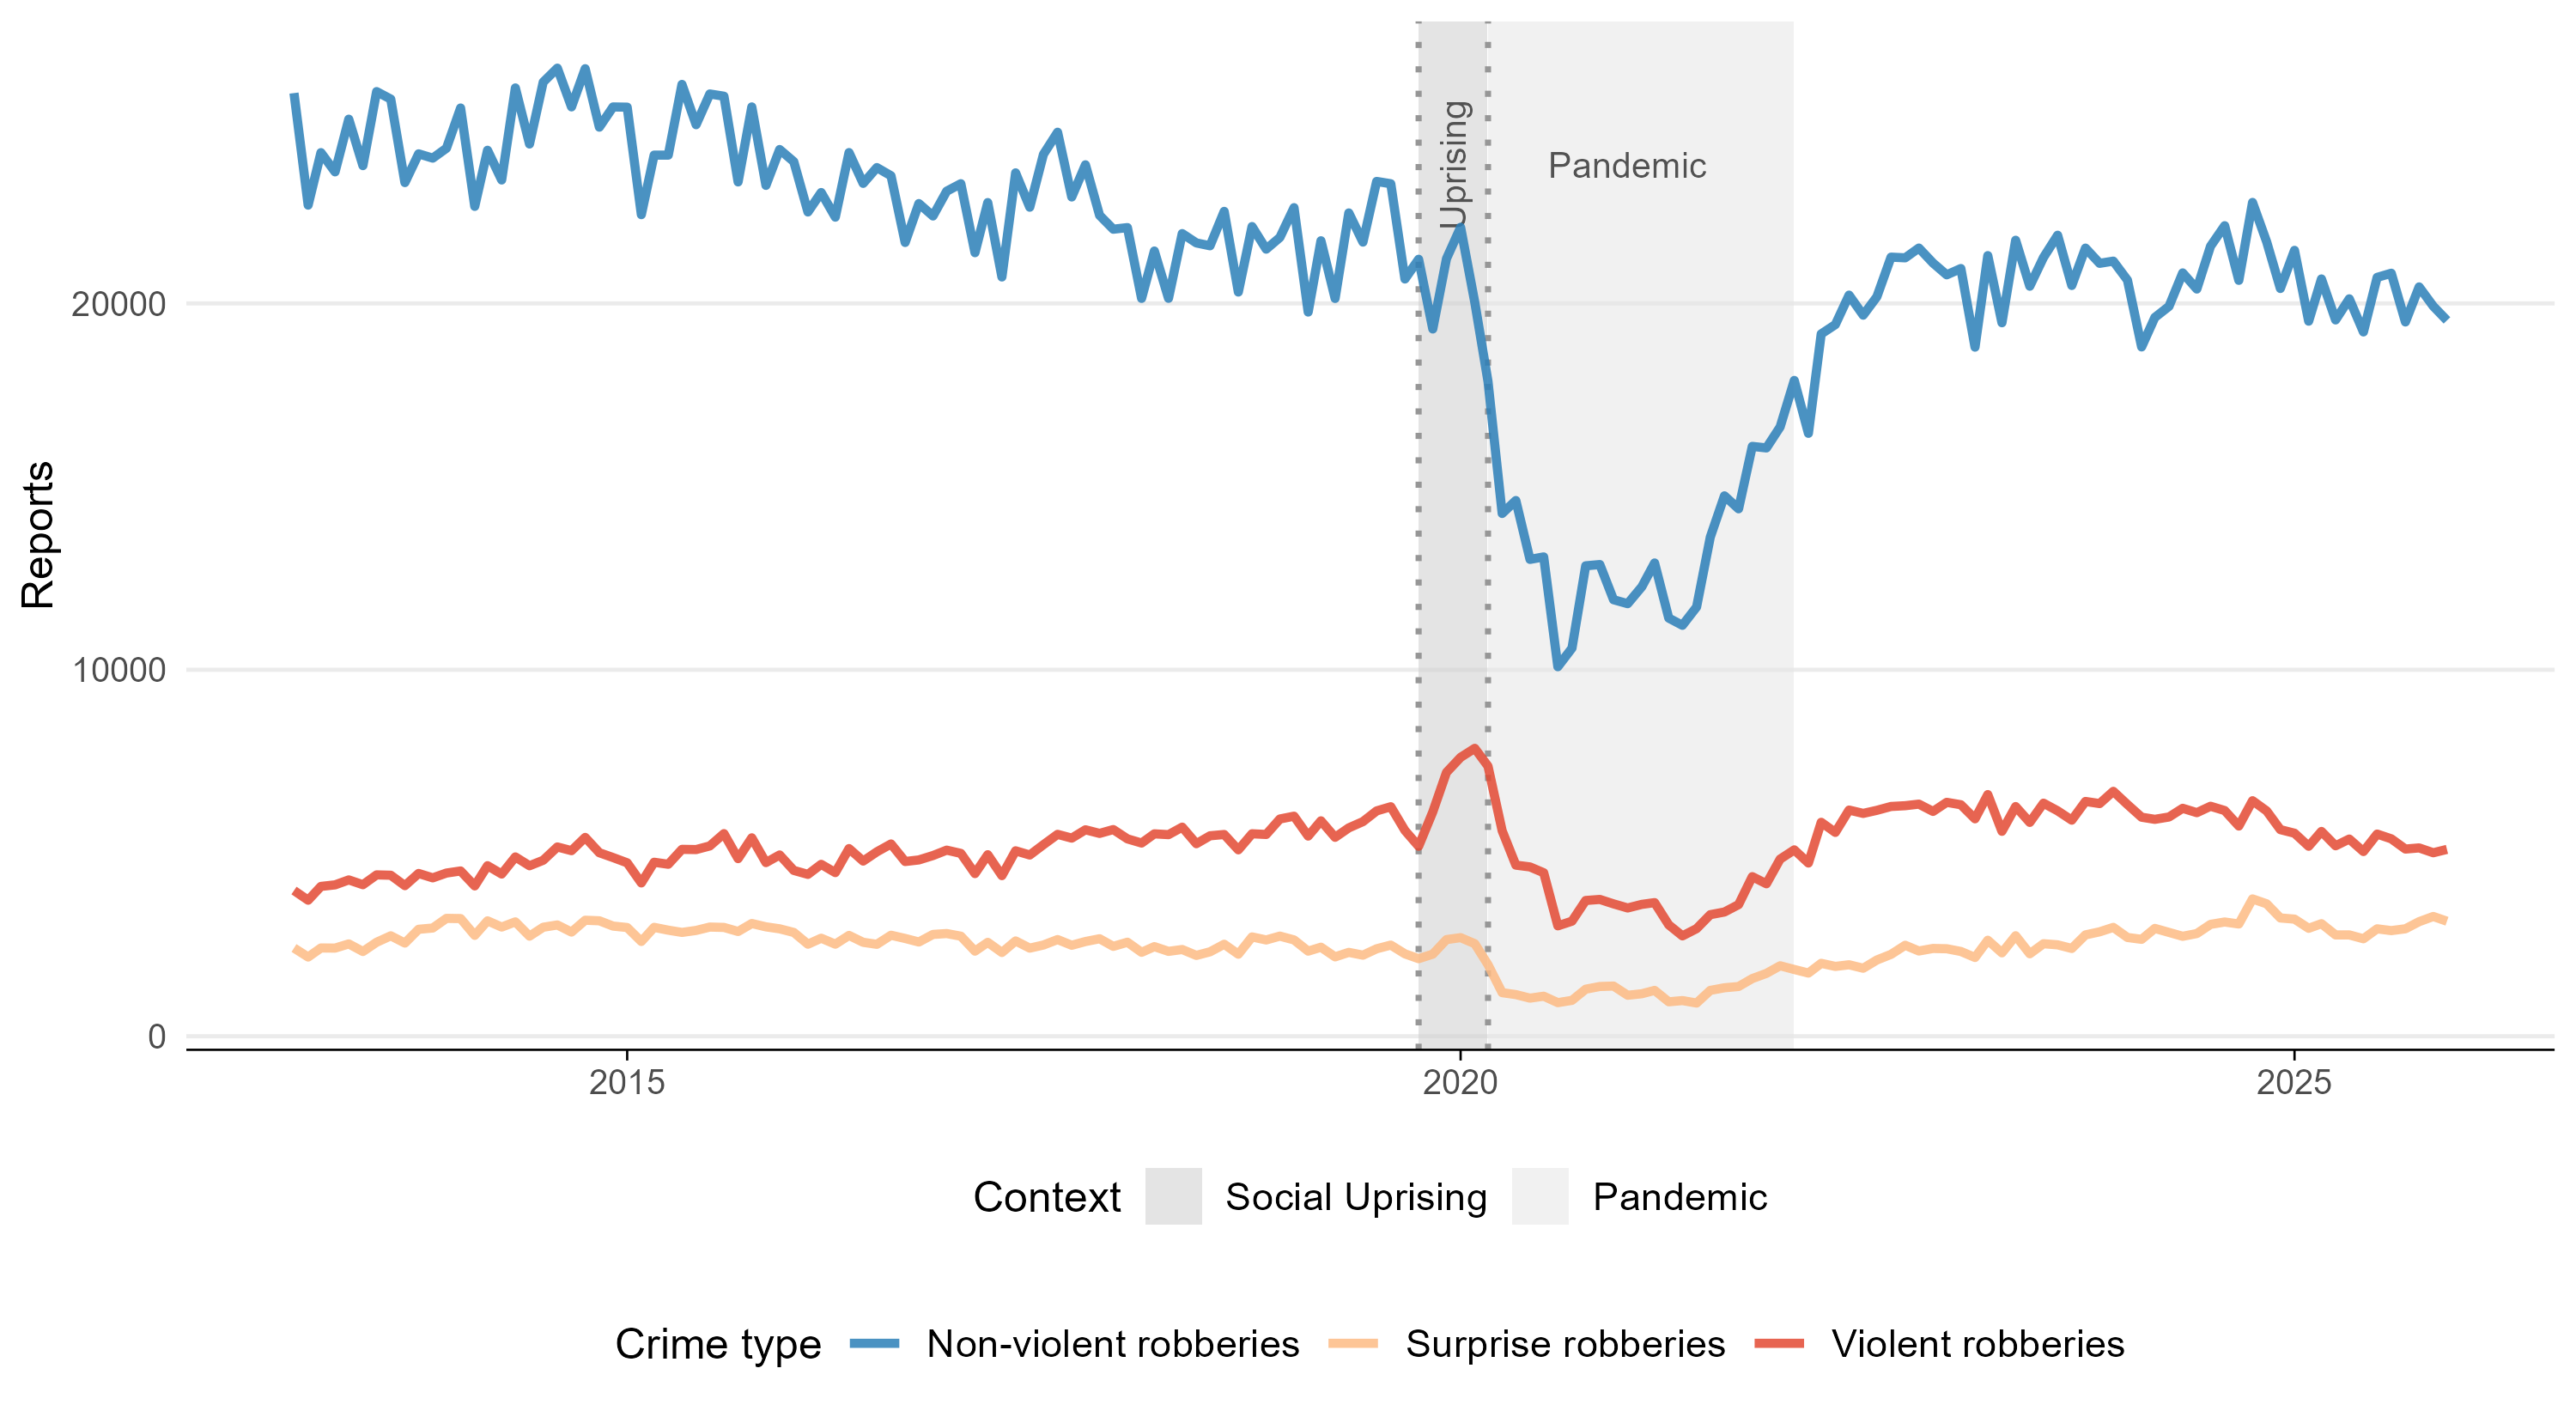
\includegraphics[width=\textwidth]{Fig1.png}
\caption{Monthly series of police cases by C3 category, Chile 2013--2025.}
\label{fig:serie}
\tablenote{The shaded bands correspond to the social uprising (Oct.\ 2019--Feb.\ 2020) and the pandemic (Mar.\ 2020--Dec.\ 2021). Source: \citet{INE2026}.}
\end{figure}

Figure~\ref{fig:serie} illustrates the distinct monthly trajectories of the three robbery types. The three episodes---uprising, pandemic, and reactivation---leave distinct footprints on each category, anticipating the analytical utility of the trichotomous classification.

Annual rates reveal the structural pattern more clearly. Confrontational robberies described an upward trajectory from 286 per 100,000 inhabitants in 2013 to 354 in 2019, collapsed to 206 during the pandemic (2021), and recovered to reach a new peak of 343 in 2023 before initiating a downward inflection in 2024--2025 (283 in 2025). Importantly, after the historical maximum of 2023, the downward inflection of 2024--2025 (283 per 100,000) anticipates the formal finding of the Poisson-QMLE model---presented in Section~\ref{sub:inferencial}---which quantifies that trend with an IRR\,=\,0.868 ($p=0.057$ by Wild Cluster Bootstrap) for Spline 4 (October 2022--December 2025).\footnote{When estimating the model with data up to December 2024, Spline 4 yields an IRR\,=\,1.039 (QMLE without WCB), indicating a practically flat trajectory in the absence of the 2025 data. The downward inflection of the main parameter emerges strictly with the incorporation of the 2025 data, which shape the downward trend.} Non-confrontational property offenses display a secular decline spanning the entire period: from nearly 1,657 per 100,000 in 2013 to 1,130 in 2024, without a significant post-pandemic recovery. This divergence in trajectories---confrontational robberies with a new downward inflection, non-confrontational property offenses in a pronounced and sustained decline---is the mechanism that generates the paradox of the growing ratio (Figure~\ref{fig:tasas}).

\begin{figure}[htbp]
\centering
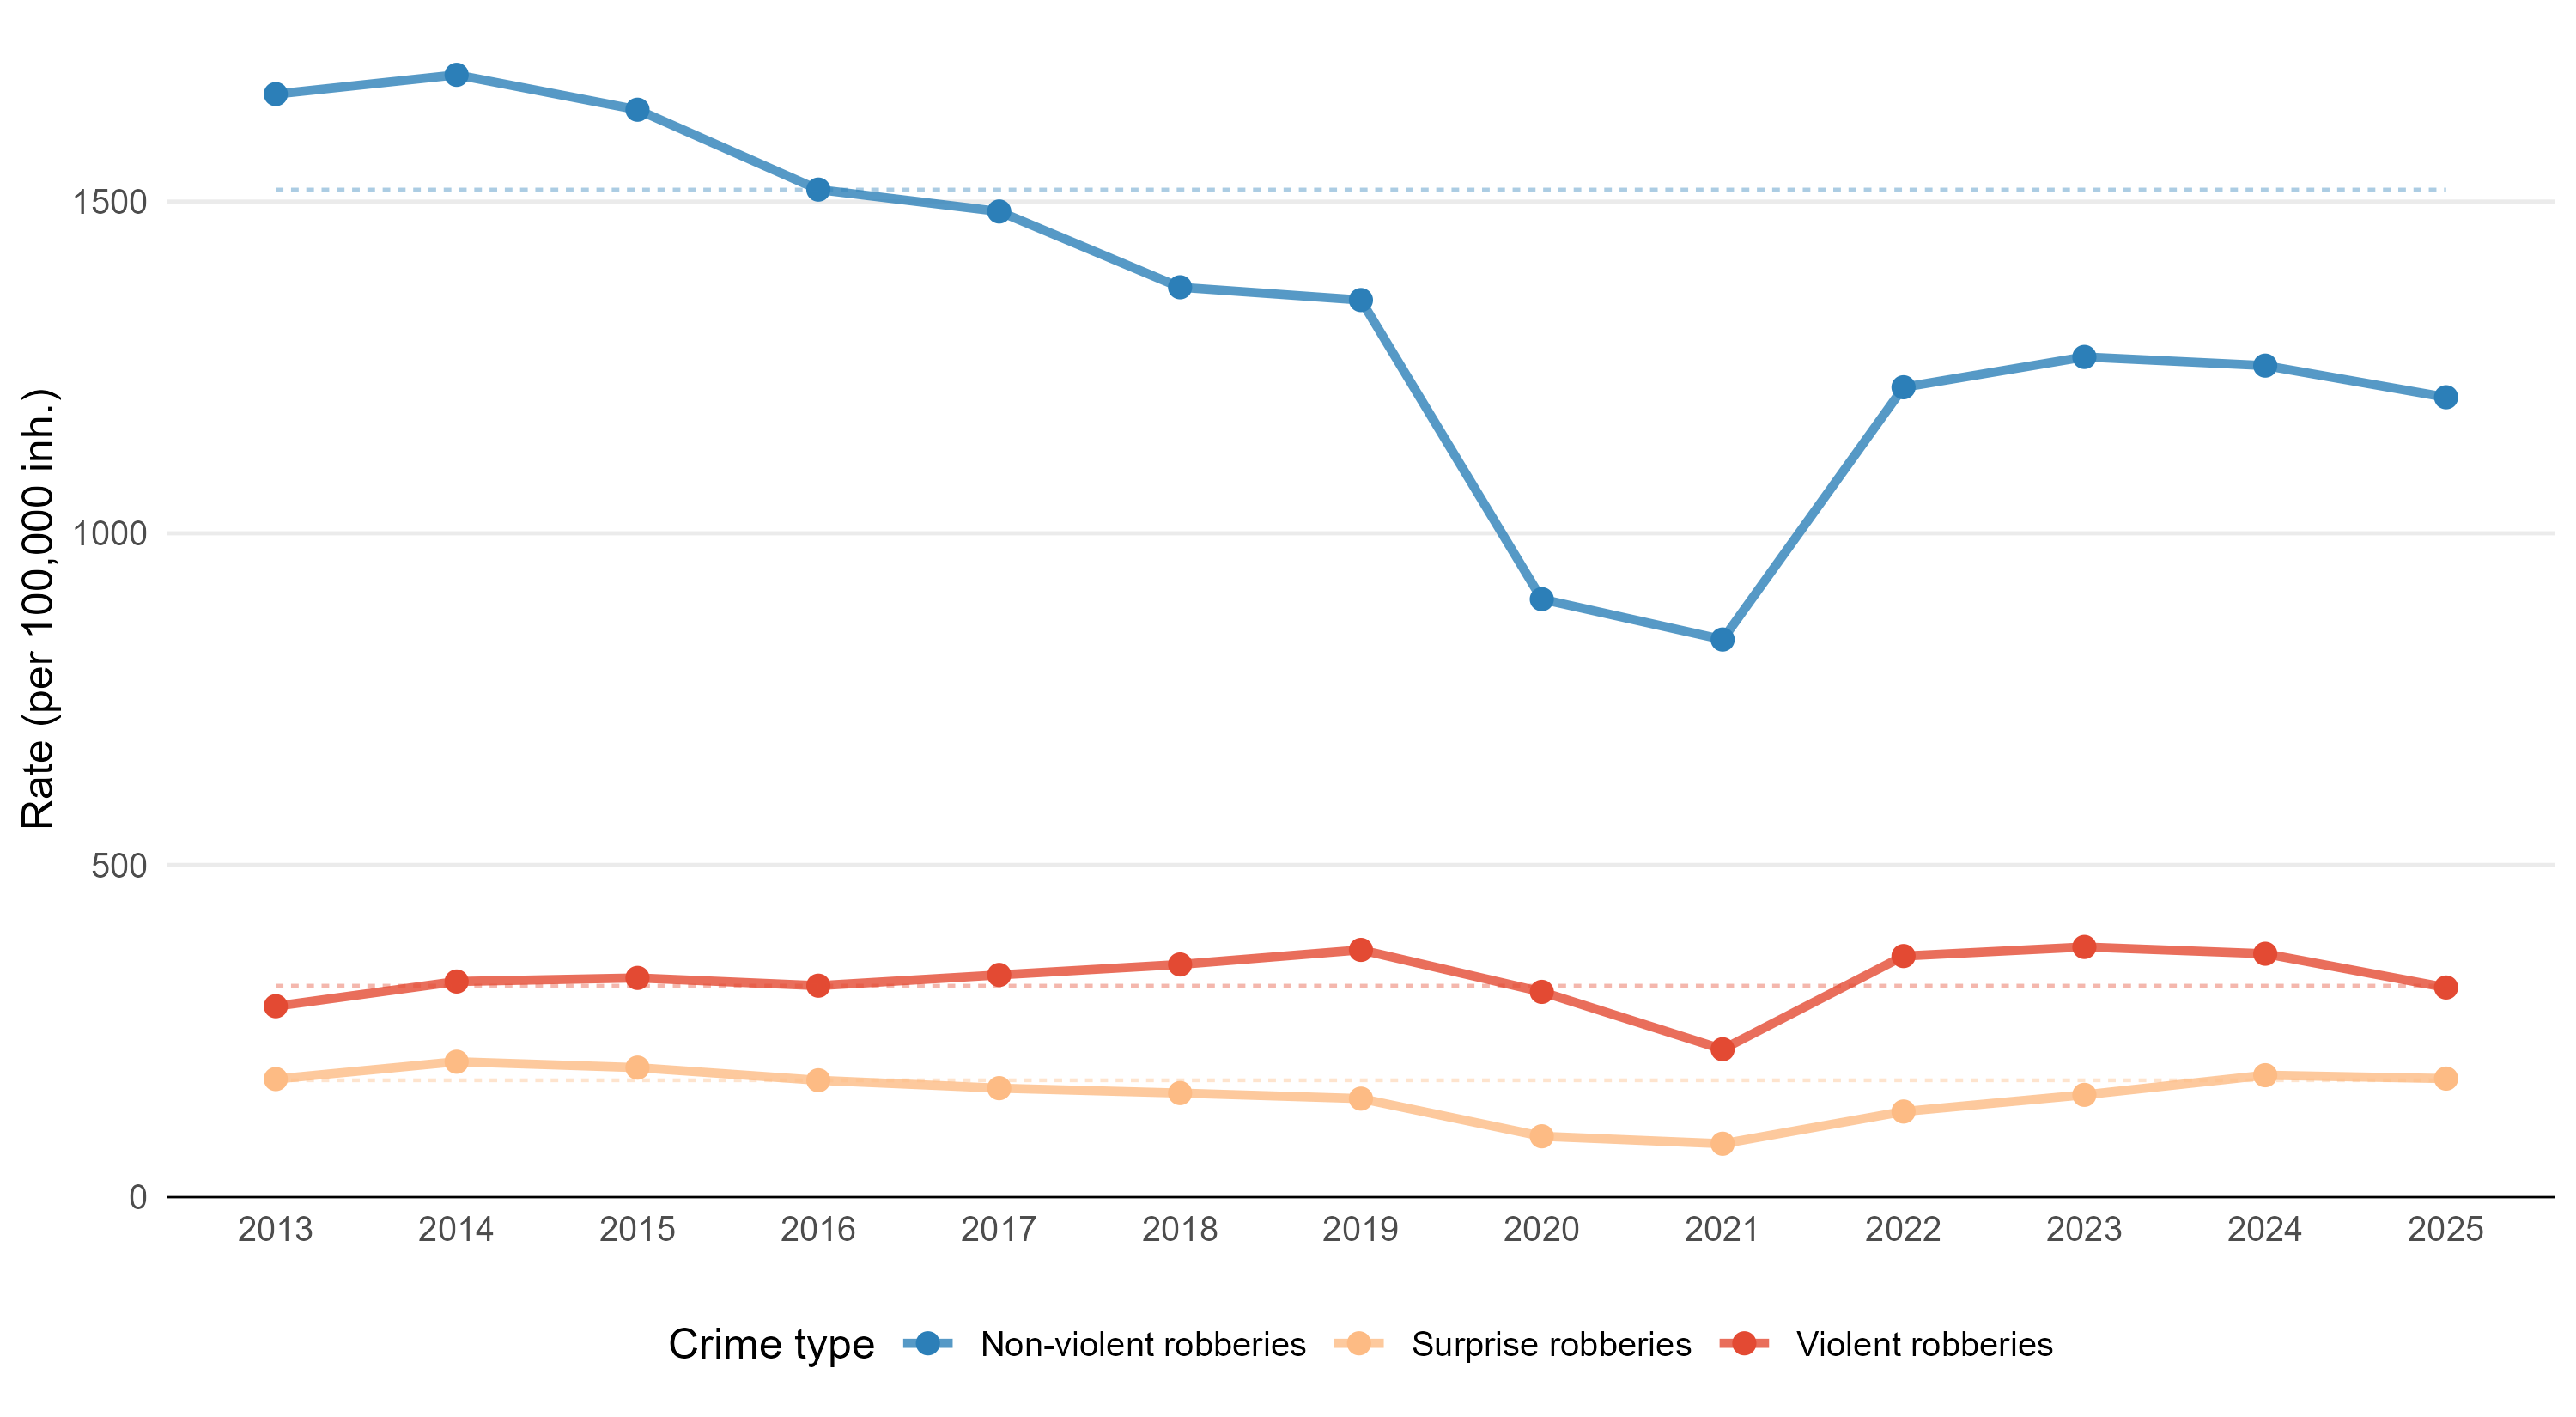
\includegraphics[width=\textwidth]{Fig2.png}
\caption{Annual rates of police cases per 100,000 inhabitants, by C3 category, Chile 2013--2025.}
\label{fig:tasas}
\tablenote{The horizontal reference line corresponds to the average of the baseline period (2016--2019). Source: \citet{INE2026}; INE Base 2024 projections (national level).}
\end{figure}

Table~\ref{tab:descriptivo} synthesizes these contrasts for the three C3 categories. Confrontational robberies presented a mean rate of 14.9 per 100,000 inhabitants in the baseline, with a transient rebound to 17.4 during the social uprising, a drop to 10.3 during the pandemic, and a recovery to 16.3 in the post-pandemic period. Snatching, with a baseline rate of 9.4, dropped sharply during the pandemic (3.9) and remained depressed in the post-pandemic period (5.8)---well below their historical level. Non-confrontational property offenses constitute the largest volume component, with a baseline rate of 106.7, falling to 60.5 during the pandemic and partially recovering to 90.9 in the post-pandemic period.

\begin{table}[htbp]
\centering
\caption{Descriptive statistics by period and C3 category (regional panel)}
\label{tab:descriptivo}
\footnotesize
\resizebox{\textwidth}{!}{
\begin{tabular}{lcrrrrrrrrrr}
\toprule
 & & \multicolumn{3}{c}{\textbf{Confrontational robberies (C3.1)}} & \multicolumn{3}{c}{\textbf{Snatching (C3.2)}} & \multicolumn{3}{c}{\textbf{Non-confrontational property offenses (C3.3)}} \\
\cmidrule(lr){3-5}\cmidrule(lr){6-8}\cmidrule(lr){9-11}
\textbf{Period} & \textbf{N} & \textbf{Mean} & \textbf{SD} & \textbf{Rate}\textsuperscript{a} & \textbf{Mean} & \textbf{SD} & \textbf{Rate}\textsuperscript{a} & \textbf{Mean} & \textbf{SD} & \textbf{Rate}\textsuperscript{a} \\
\midrule
Pre-baseline (2013--2015)      & 36 & 290.3 &  719.5 &  15.5 & 177.4 &  364.1 &  11.7 & 1,538.5 & 2,565.7 & 124.3 \\
Baseline (2016--Sep.\ 2019)    & 45 & 330.0 &  875.2 &  14.9 & 156.4 &  328.6 &   9.4 & 1,393.1 & 2,282.0 & 106.7 \\
Uprising (Oct.\ 2019--Feb.\ 2020) &  5 & 424.7 & 1,200.8 &  17.4 & 152.6 &  348.8 &   8.2 & 1,297.9 & 2,111.1 &  95.6 \\
Pandemic (Mar.\ 2020--Dec.\ 2021)  & 22 & 247.2 &  698.4 &  10.3 &  79.0 &  198.2 &   3.9 &   835.3 & 1,331.9 &  60.5 \\
Post-pandemic (2022--2025)         & 48 & 366.6 &  939.1 &  16.3 & 166.2 &  484.4 &   5.8 & 1,275.8 & 1,918.5 &  90.9 \\
\bottomrule
\end{tabular}
}
\tablenote{Panel of 16 regions $\times$ N months. Mean and SD calculated on region-month observations. \textsuperscript{a} Average rate per 100,000 inhabitants at the regional level. Source: \citet{INE2026}; SERMIG; INE Base 2017 projections.}
\end{table}

Disaggregating the empirical data (Table~\ref{tab:cum}), the two crimes that dominate confrontational robberies---robbery with intimidation (64.3\% of the group) and robbery with violence (28.7\%)---display post-pandemic rates $-22.9\%$ and $-8.3\%$ below the baseline period, respectively. Together they account for 93\% of the group, and their downward trend is the most robust piece of the descriptive analysis. Vehicle theft via violence or intimidation (CUM 867) appears in the system with substantial volume only since 2020, representing 6.6\% of the group over the full period; therefore, its comparison uses the 2018--2020 period as a reference baseline. The only offense demonstrating sustained real growth within the group is robbery with victim retention or severe injury (CUM 862), showing a 263\% increase between periods---but from a very low base (less than 0.1\% of the group): 83 cases in 2022 versus 283 in 2025. Among non-confrontational property offenses, the decline is generalized: the most pronounced corresponds to robbery in an inhabited place ($-35.0\%$) and theft of 0.5 to 4 UTM ($-25.7\%$).

\begin{table}[htbp]
\centering
\caption{Intra-category composition: main CUMs of the C3 classification (2013--2025)}
\label{tab:cum}
\footnotesize
\resizebox{\textwidth}{!}{
\begin{tabular}{lrp{4.5cm}rrrr}
\toprule
\textbf{Cat.} & \textbf{CUM} & \textbf{Description} & \textbf{Total N} & \textbf{\% group} & \textbf{Base rate\textsuperscript{a}} & \textbf{$\Delta$\%\textsuperscript{b}} \\
\midrule
\multicolumn{7}{l}{\textit{Confrontational robberies}} \\
 & 802 & Robbery with intimidation                         & 519,171 & 64.3 & 238.5 & $-$22.9 \\
 & 803 & Robbery with violence                              & 232,073 & 28.7 &  97.7 & $-$8.3  \\
 & 867 & Vehicle theft with violence/intimidation\textsuperscript{c} &  53,130 & 6.6 & 10.5\textsuperscript{d} & $+$389 \\
 & 828 & Robbery with rape                            &   1,470 &  0.2 &  0.66 & $-$14.1 \\
 & 862 & Robbery with victim retention or severe injuries &   992 &  0.1 &  0.24 & $+$263  \\
 & 827 & Robbery with homicide                              &     320 &  0.0 &  0.10 & $+$55   \\
 & 861 & Robbery with severe injuries                        &     175 &  0.0 &  0.09 & $+$17   \\
 & 829 & Robbery with castration, mutilation, or severe injuries &  15  &  0.0 & 0.005 & $+$71   \\
\midrule
\multicolumn{7}{l}{\textit{Snatching}} \\
 & 804 & Surprise robbery (snatching)                     & 382,445 & 100.0 & 158.2 & $-$8.0 \\
\midrule
\multicolumn{7}{l}{\textit{Non-confrontational property offenses}} \\
 & 808 & Robbery in national property of public use\textsuperscript{e}   & 739,657 & 22.7 & 317.3 & $-$18.9 \\
 & 809 & Robbery in inhabited place        & 589,940 & 18.1 & 268.9 & $-$35.0 \\
 & 847 & Theft 4--40 UTM               & 544,015 & 16.7 & 235.5 & $-$15.4 \\
 & 810 & Robbery in uninhabited place     & 480,777 & 14.7 & 206.6 & $-$15.8 \\
 & 848 & Theft 0.5--4 UTM              & 403,089 & 12.3 & 174.4 & $-$25.7 \\
 & 831 & Vehicle theft without violence  & 350,990 & 10.8 & 137.0 & $-$4.8  \\
 & --- & Rest                          &    --- &  4.7 &   --- & variable \\
\bottomrule
\end{tabular}
}
\tablenote{\textsuperscript{a} Average rate per 100,000 inh.\ in the baseline period (2016--2019). \textsuperscript{b} Percentage change between base rate (2016--2019) and post-pandemic rate (2022--2025). \textsuperscript{c} Includes \textit{portonazos} and \textit{encerronas}. \textsuperscript{d} Exception: this code records significant volume only since 2020. The base rate is calculated over 2018--2020 ($\bar{x}_{\text{annual}} = 10.5$ per 100,000), and $\Delta$\% compares that period with 2022--2025. \textsuperscript{e} Covers theft of vehicle parts and goods left inside vehicles (e.g.\ bags, personal belongings) in public roads and spaces (\textit{bien nacional de uso p\'ublico}). 1~UTM\,=\,69,542~CLP as of December 2025 (USD~76.32 at 911.18~CLP/USD). Total N = police cases 2013--2025. Source: \citet{INE2026}; SERMIG; INE Base 2017 projections.}
\end{table}

The monthly ratio of confrontational robberies/(confrontational + non-confrontational property offenses), once seasonally adjusted and smoothed via a local polynomial regression,\footnote{Local weighted least squares smoothing (LOESS): estimates a weighted regression at each point over the temporally closest observations. The parameter \texttt{span}\,=\,0.2 equates to using 20\% of the observations as a smoothing window.} ascends almost monotonically from 14.7\% in April 2015 to a historical peak of 21.6\% in January 2024. Its function is exclusively descriptive: it reveals the underlying trend filtered of short-term seasonal noise, without constituting a formal hypothesis test. The resulting curve is consistent with---but conceptually independent of---the formal Bai-Perron breaks. The Bai-Perron algorithm, selecting $m=4$ optimal breaks by the Bayesian information criterion, identifies four successive inflections: Q1 in April 2015 (14.7\%), Q2 in August 2017 (17.1\%), Q3 in October 2019 (18.4\%), and Q4 in January 2024 (21.6\%).\footnote{Estimating the algorithm with data up to December 2024---without incorporating year 2025---shifts the fourth optimal break to April 2021 (IRR of the posterior segment = 1.04, QMLE), capturing the strong post-pandemic reactivation. The January 2024 break emerges solely upon incorporating the 2025 data, establishing that level as a downward inflection point of the ratio.} Each break marks a new step in the ratio, yet the mechanism sustaining them is not the growth of confrontational robberies, but the sharper contraction of non-confrontational property offenses in the denominator. This paradox---a growing ratio alongside decreasing absolute volume---constitutes the central finding of the work. Figure~\ref{fig:ratio} visually represents this paradox: the LOESS curve illustrates an almost monotonically rising trend intersected by four sequential Bai-Perron segmentations.

\begin{figure}[htbp]
\centering
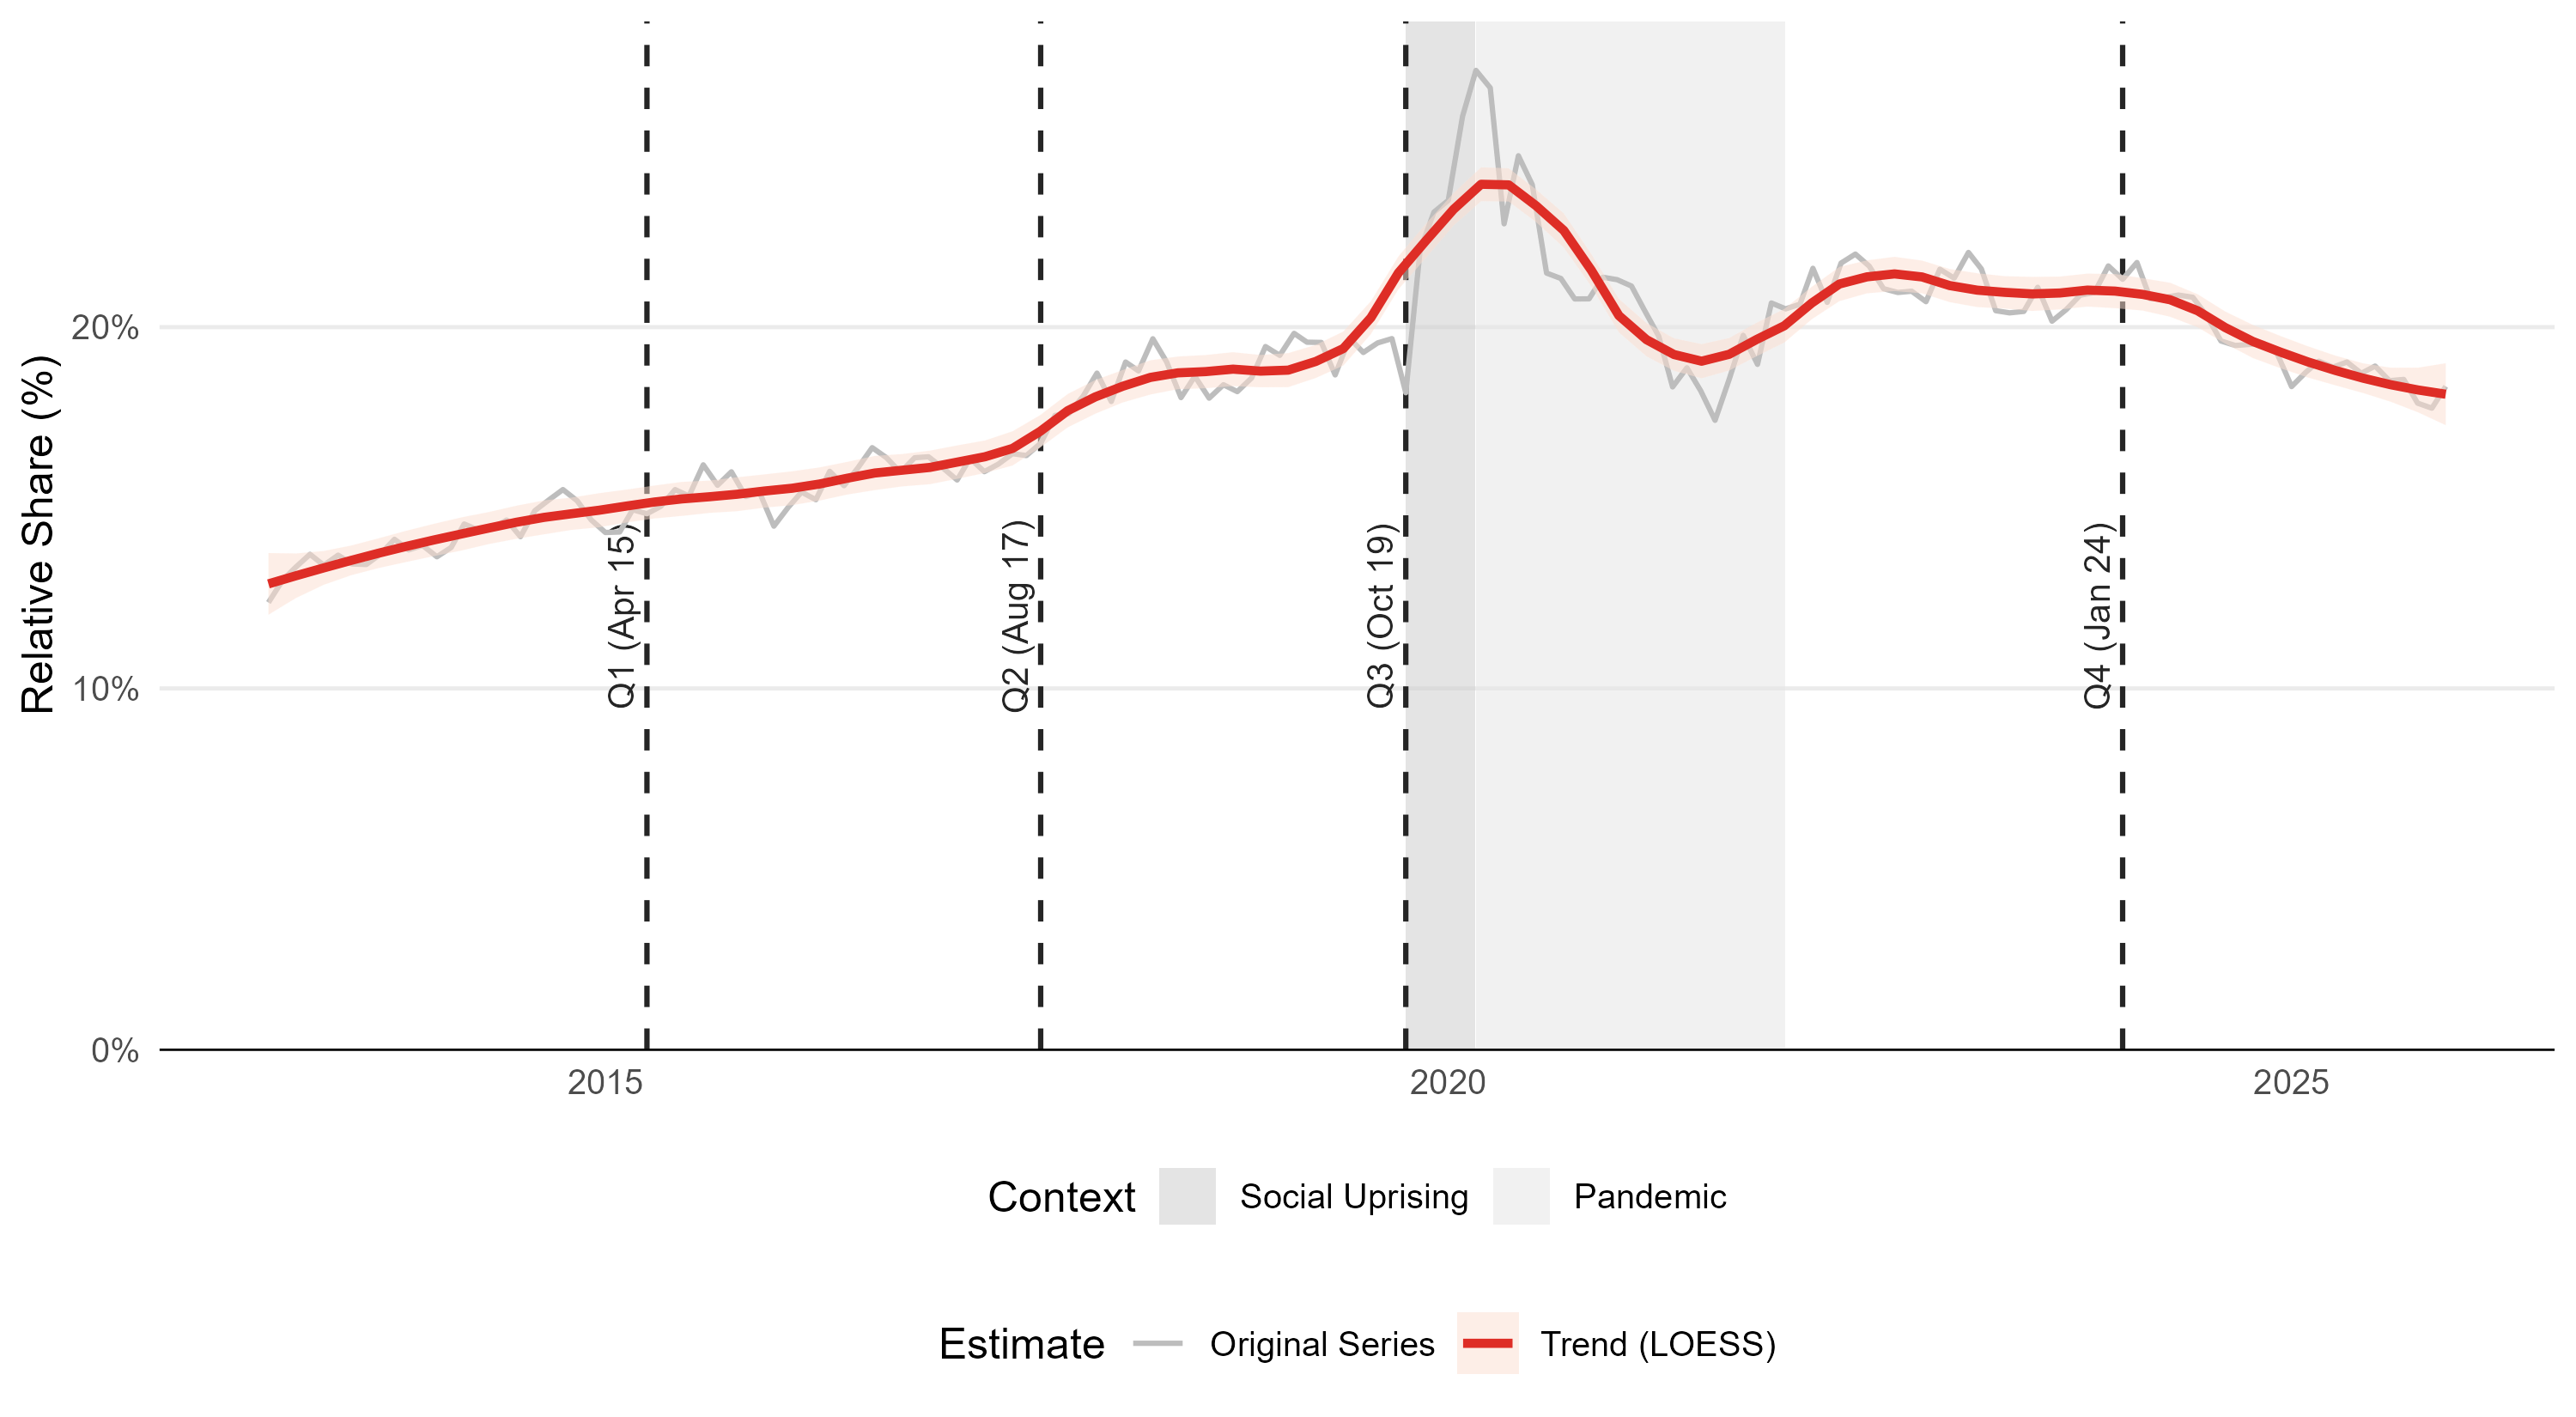
\includegraphics[width=\textwidth]{Fig3.png}
\caption{Monthly ratio of confrontational robberies/(confrontational + non-confrontational property offenses) with Bai-Perron breaks.}
\label{fig:ratio}
\tablenote{The vertical dashed lines mark the four optimal breaks by BIC: Q1 = Apr.\ 2015 (14.7\%); Q2 = Aug.\ 2017 (17.1\%); Q3 = Oct.\ 2019 (18.4\%); Q4 = Jan.\ 2024 (21.6\%). Seasonally adjusted series. Source: \citet{INE2026}.}
\end{figure}

The spatial dimension of the change reinforces this interpretation. The log-ratio between the average rate of the recent period (2022--2025) and the baseline (2016--2019) reveals that the phenomenon is not geographically uniform (Figure~\ref{fig:mapatasa}). The Northern macro-zone---particularly Arica y Parinacota and Tarapac\'a---exhibits the largest relative increments, mapping coherently against mounting migratory pressures accumulated since 2018 alongside reorganized routes managed by organized crime operating across that border. By contrast, several regions within the Southern macro-zone---Biob\'io, La Araucan\'ia, Maule---illustrate negative log-ratio values: their rates in 2022--2025 are below the 2016--2019 baseline level. This apparent paradox is consistent with their trajectory in the CUSUM tests---presented below in Section~\ref{sub:regional}---where these regions reached a relatively early peak (structural breaks detected around 2017--2018) and then converged downward. The Metropolitan Region hovers around zero, reflecting a post-pandemic recovery that converges toward the baseline level without surpassing it persistently. Ultimately, the map illustrates that the downward inflection of Spline~4 does not operate homogeneously across the territory: while the North still exhibits positive balances compared to 2016--2019, the South already records negative ones, and the national aggregate is the result of that partial compensation.

\begin{figure}[htbp]
\centering
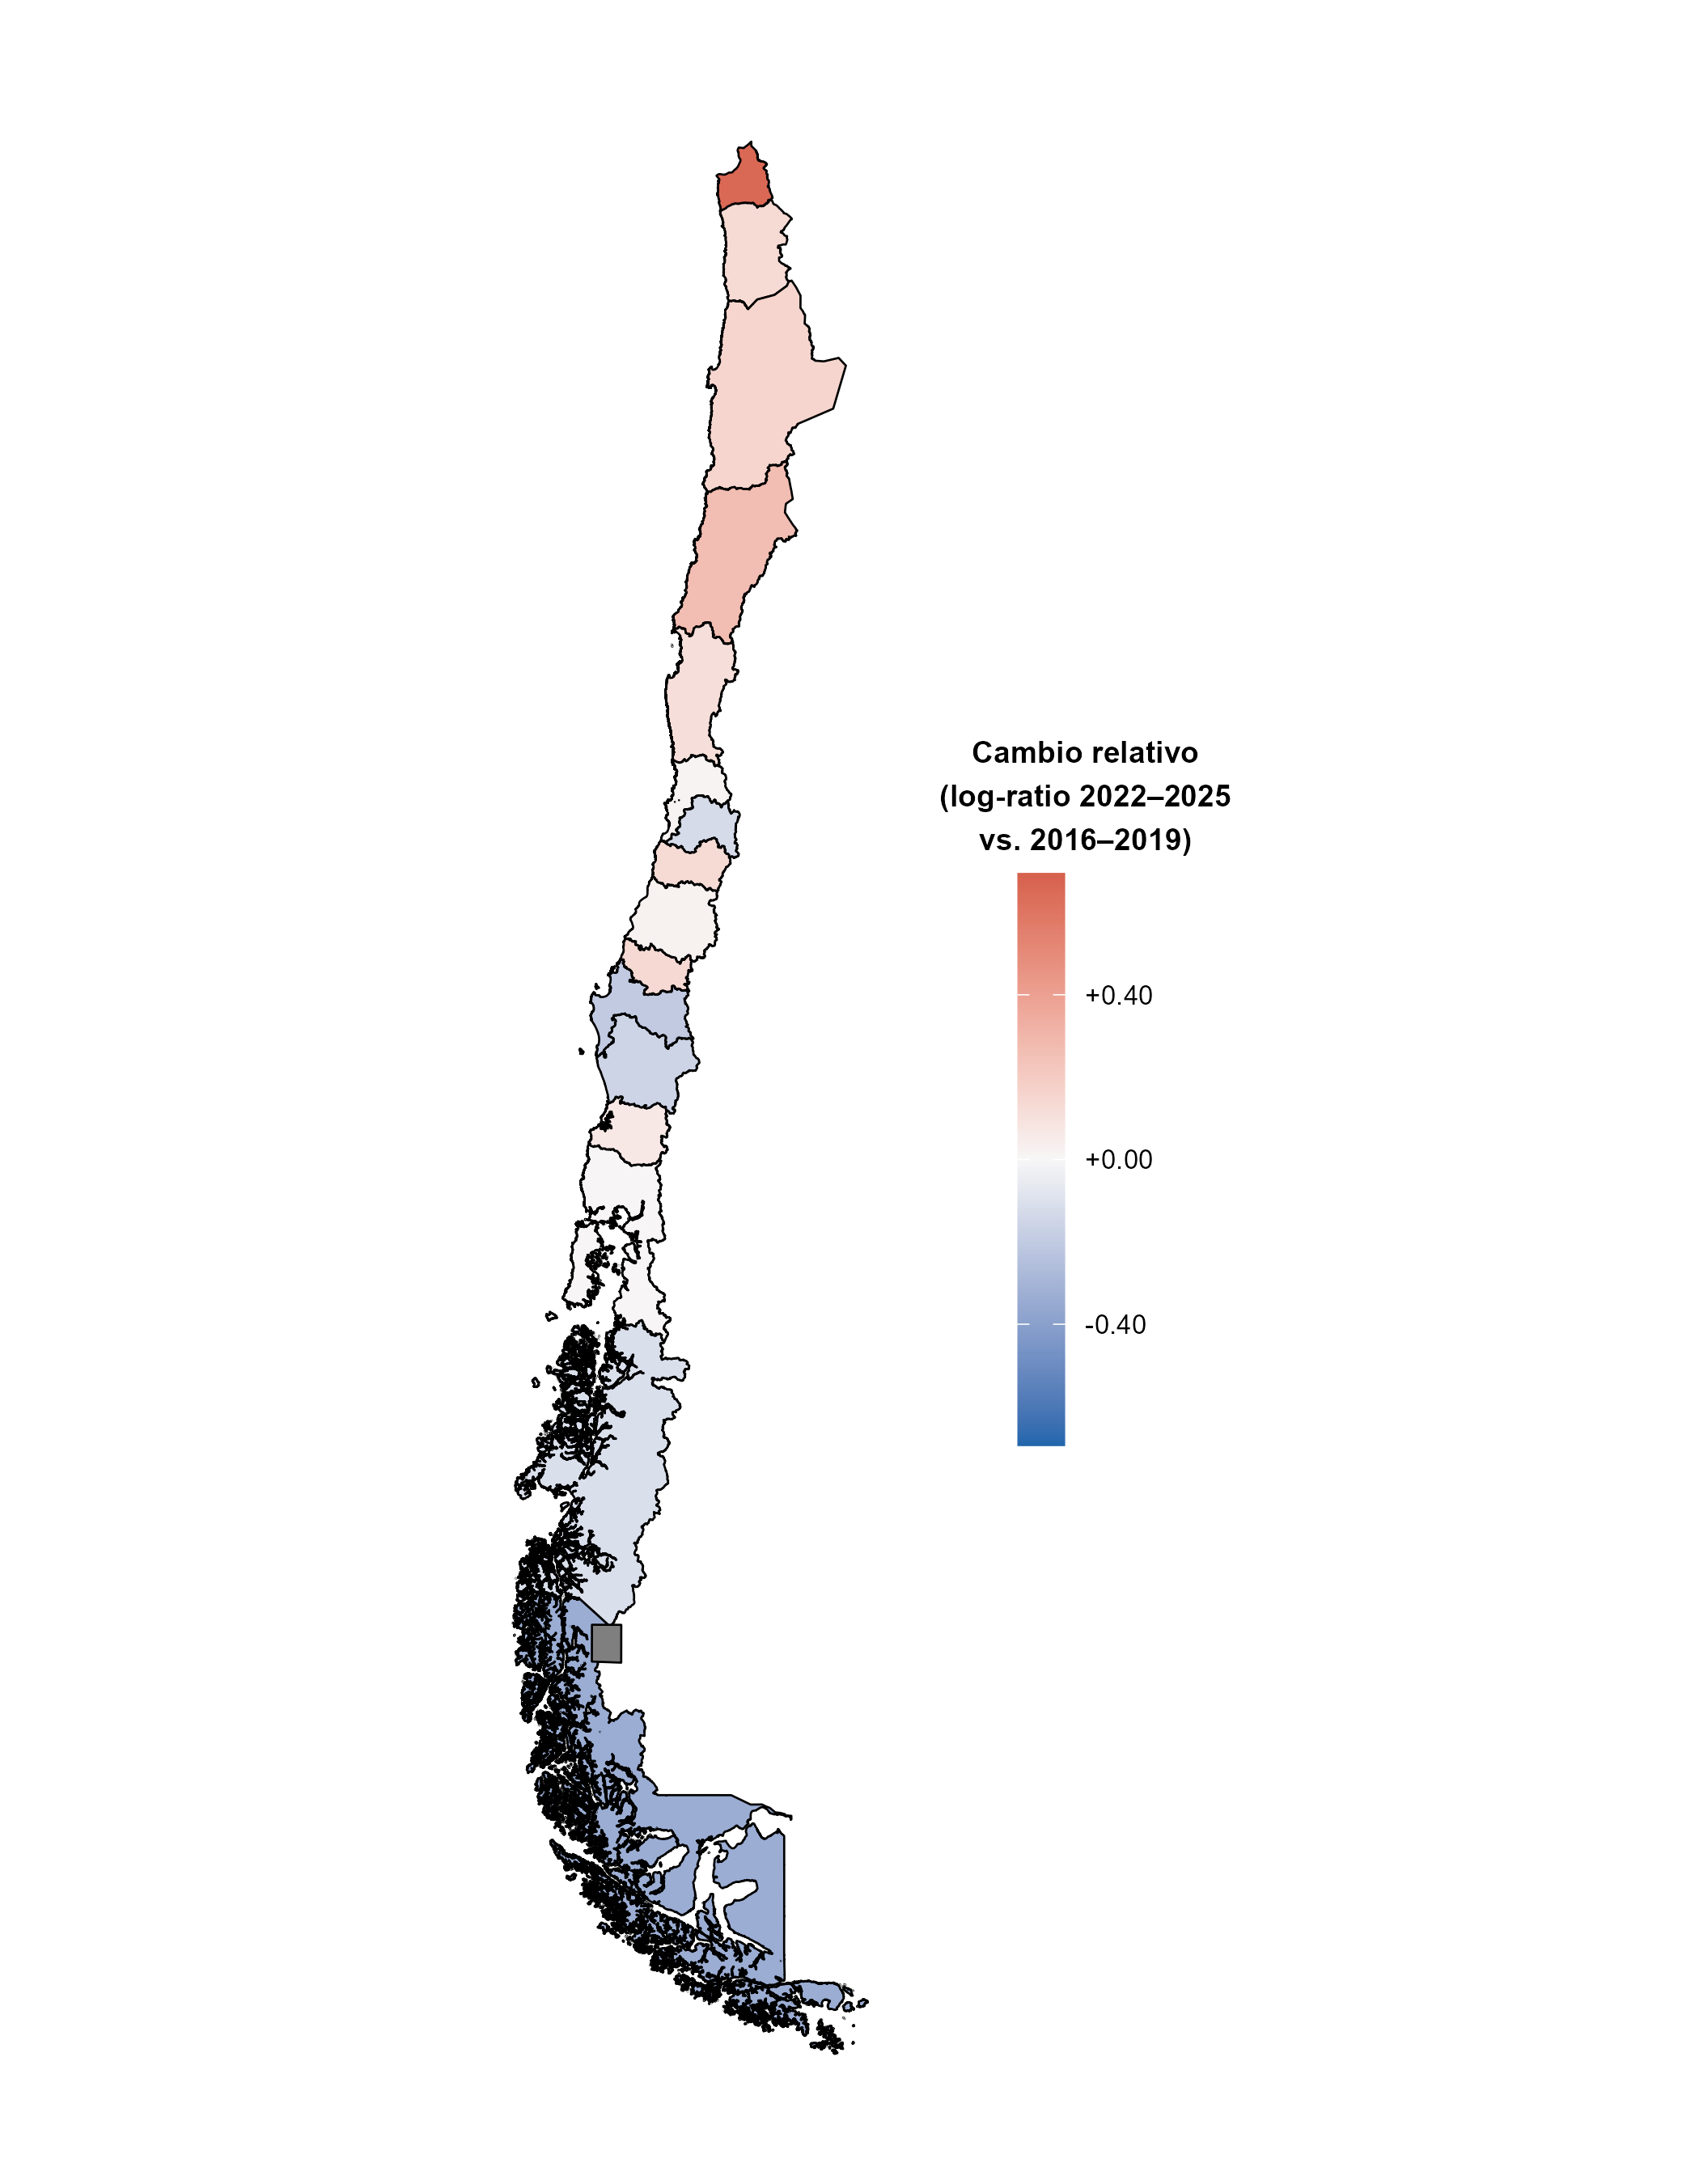
\includegraphics[width=0.72\textwidth]{Fig5.png}
\caption{Relative change in confrontational robbery rates by region: log-ratio of the recent period (2022--2025) relative to the baseline period (2016--2019).}
\label{fig:mapatasa}
\tablenote{Positive values (red) denote regions where the rate in 2022--2025 surpasses that of 2016--2019; negative values (blue) indicate regions with a lower rate in the recent period. The log-ratio captures proportional change while neutralizing differences in absolute scale between regions---a region with a low rate and one with a high rate that double are represented identically. Source: \citet{INE2026}; SERMIG; INE Base 2017 projections.}
\end{figure}

\subsection{Main Model: Long-term Trend}
\label{sub:inferencial}

Table~\ref{tab:poisson} reports the results of the Poisson-QMLE model for the three C3 categories. For confrontational robberies, the social uprising produced a transient increase of 15.5\% (IRR\,=\,1.155; $p<0.001$), consistent with the hypothesis that the protest climate facilitated direct confrontation crimes. Snatching increased by 6.9\% (IRR\,=\,1.069; $p<0.001$). In contrast, non-confrontational property offenses did not react to the uprising (IRR\,=\,0.996; $p=0.761$): their dynamics respond to structural factors of opportunity, not to social conflict. The pandemic contracted all types of property crime: confrontational robberies by 34.9\% (IRR\,=\,0.651) and non-confrontational property offenses by 35.3\% (IRR\,=\,0.647). Snatching experienced the most pronounced drop (-42.4\%, IRR\,=\,0.576), reflecting their absolute dependence on agglomeration and urban circulation.

The temporal evolution of the baseline trend---captured by the spline---exhibits radically different behaviors according to crime type. Confrontational robberies display positive point estimates across the first three segments: Spline~1 (2013--2016: IRR\,=\,1.178, $p=0.201$), Spline~2 (2016--2019: IRR\,=\,1.136, $p=0.087$), and Spline~3 (2019--2022: IRR\,=\,1.187, $p<0.001$)---though only Spline~3 reaches conventional significance, consistent with the progressively consolidating upward trend from 2013 to 2022. However, the trend reverses in Spline~4 (October 2022--December 2025), which registers a downward inflection with an IRR of 0.868. This inflection falls on the edge of conventional statistical significance ($p=0.057$), indicating that the phenomenon is suggestive but requires caution given the reduced number of clusters ($G=16$). 

Non-confrontational property offenses display an entirely distinct structural trajectory. Their splines show constant and progressive declines across all four segments: Spline~1 (IRR\,=\,0.718, $p<0.001$), Spline~2 (IRR\,=\,0.685, $p<0.001$), Spline~3 (IRR\,=\,0.656, $p<0.001$), and Spline~4 (IRR\,=\,0.648, $p<0.001$). The monotonically decreasing sequence represents a cumulative reduction of 35.2\% relative to the initial trend level. This structural decline operates independently of the transient shocks and reflects a sustained contraction in opportunities for contactless theft, linked to transformations in residential security and retail digitization.

Snatching exhibit an erratic behavior conditioned by their dependence on circulation. Following significant contractions in Splines 1 and 2 (IRR\,=\,0.668 and 0.635, respectively), the trajectory approached unity in Spline~3 (IRR\,=\,0.968, $p=0.882$)---already statistically indistinct from a flat trend---and stabilized into the post-pandemic reactivation, with a non-significant Spline~4 (IRR\,=\,0.861, $p=0.574$). The divergence in these paths validates the relevance of the trichotomous classification: the apparent stability of aggregated property crime masks highly divergent internal compositions.

\begin{table}[htbp]
\centering
\caption{Poisson-QMLE model with Wild Cluster Bootstrap: main results (C3)}
\label{tab:poisson}
\footnotesize
\resizebox{\textwidth}{!}{
\begin{tabular}{l@{\hskip 3mm}ccc@{\hskip 4mm}ccc@{\hskip 4mm}ccc}
\toprule
 & \multicolumn{3}{c}{\textbf{Confrontational robberies}} & \multicolumn{3}{c}{\textbf{Snatching}} & \multicolumn{3}{c}{\textbf{Non-confrontational}} \\
\cmidrule(lr){2-4}\cmidrule(lr){5-7}\cmidrule(lr){8-10}
\textbf{Term} & IRR & 95\% CI & $p$ & IRR & 95\% CI & $p$ & IRR & 95\% CI & $p$ \\
\midrule
$D^{\text{est}}$ & 1.155 & [1.119, 1.192] & $<$.001 & 1.069 & [1.031, 1.108] & $<$.001 & 0.996 & [0.971, 1.022] & .761 \\
$D^{\text{pan}}$ & 0.651 & [0.621, 0.682] & $<$.001 & 0.576 & [0.547, 0.606] & $<$.001 & 0.647 & [0.628, 0.665] & $<$.001 \\
\midrule
Spline 1    & 1.178 & [0.917, 1.513] & .201 & 0.668 & [0.619, 0.722] & $<$.001 & 0.718 & [0.673, 0.767] & $<$.001 \\
Spline 2    & 1.136 & [0.982, 1.315] & .087 & 0.635 & [0.462, 0.873] & .005 & 0.685 & [0.568, 0.826] & $<$.001 \\
Spline 3    & 1.187 & [1.116, 1.264] & $<$.001 & 0.968 & [0.634, 1.480] & .882 & 0.656 & [0.570, 0.754] & $<$.001 \\
\textbf{Spline 4} & \textbf{0.868} & \textbf{[0.751, 1.004]} & \textbf{.057} & 0.861 & [0.511, 1.450] & .574 & \textbf{0.648} & \textbf{[0.580, 0.723]} & $<$.001 \\
\midrule
Obs. & 2,496 & & & 2,496 & & & 2,496 & & \\
\bottomrule
\end{tabular}
}
\tablenote{IRR = exp($\hat{\beta}$). 95\% CI via WCB inversion (Webb weights, $B=9,999$, $G=16$). $D^{\text{est}}$: social uprising dummy (Oct.\ 2019--Feb.\ 2020). $D^{\text{pan}}$: pandemic dummy (Mar.\ 2020--Dec.\ 2021). Spline~1--4: restricted cubic spline with knots at P25 ($\approx$ Apr.\ 2016), P50 ($\approx$ Jun.\ 2019), and P75 ($\approx$ Sep.\ 2022). All models include regional fixed effects and monthly seasonality dummies. Offset: $\log$(corrected monthly population).}
\end{table}

\subsection{Structural Breaks and Territorial Heterogeneity}
\label{sub:regional}

The CUSUM-GLM tests detect structural breaks in the long-term trend of confrontational robberies in 12 of the 16 regions ($p$-FDR\,$<$\,0.05). Counting by year of maximum accumulation: one region broke in 2016 (Ays\'en), two in 2017 (Maule, Magallanes), two in 2018 (La Araucan\'ia, Biob\'io), one in 2020 (Metropolitan Region), five in 2021 (Arica y Parinacota, Atacama, O'Higgins, Coquimbo, \~Nuble), and one in 2023 (Tarapac\'a). The concentration of five simultaneous breaks in 2021 is consistent with the hypothesis that the pandemic-plus-reactivation period imposed the greatest simultaneous structural pressure on regional criminal patterns, although it is worth noting that five of the twelve breaks preceded 2020, predating the period most frequently cited by authorities as ``the most critical year'' for citizen security. Table~\ref{tab:cusum} details the dates of maximum accumulation for each territory, revealing that the structural alteration was not a single, synchronous shock across the country. 

The first group, with pre-pandemic inflections, spans the Austral and Southern macro-zones: Ays\'en (February 2016) records the earliest detected break in the dataset, followed by Magallanes (August 2017), Maule (April 2017), Biob\'io (August 2018), and La Araucan\'ia (July 2018). These inflections precede the social uprising by more than two years, indicating local processes independent of the national shock. In La Araucan\'ia and Biob\'io, this period coincides with the escalation of the Mapuche territorial conflict---arson attacks, machinery destruction, and clashes with law enforcement---which generated a local context of heightened predisposition to violent crime. In Ays\'en, Magallanes, and Maule, early inflections reflect local dynamics of criminal network recomposition and, to a lesser extent, internal migration flows. 

The second group, with breaks occurring during the pandemic and reactivation, encompasses the majority of regions---Metropolitan Region (July 2020), Atacama (August 2021), O'Higgins (September 2021), Coquimbo (September 2021), Arica y Parinacota (July 2021), and \~Nuble (August 2021)---clustering between July 2020 and September 2021. The combination of mobility restrictions and subsequent reactivation reorganized criminal patterns profoundly enough to generate statistically detectable breaks. 

The third group comprises late inflections strictly confined to Tarapac\'a (August 2023): the intensity of migration across the northern border and the reconfiguration of organized crime routes explain this delay. Four regions---Antofagasta, Valpara\'iso, Los Lagos, and Los R\'ios---show no evidence of a significant break.

\begin{table}[htbp]
\centering
\caption{CUSUM-GLM tests: structural break in confrontational robberies by region}
\label{tab:cusum}
\footnotesize
\resizebox{\textwidth}{!}{
\begin{tabular}{llccc}
\toprule
\textbf{Region} & \textbf{Macro-zone} & \textbf{p-value} & \textbf{p-FDR} & \textbf{Estimated break} \\
\midrule
R15 --- Arica y Parinacota & North   & $<$.001  & $<$.001 & Jul.\ 2021 \\
R8 --- Biob\'io            & South     & $<$.001  & $<$.001 & Aug.\ 2018 \\
R9 --- La Araucan\'ia      & South     & $<$.001  & $<$.001 & Jul.\ 2018 \\
R7 --- Maule               & Central  & $<$.001  & $<$.001 & Apr.\ 2017 \\
R3 --- Atacama             & North   & $<$.001  & $<$.001 & Aug.\ 2021 \\
R6 --- O'Higgins           & Central  & $<$.001  & $<$.001 & Sep.\ 2021 \\
R13 --- Metropolitan      & RM      & $<$.001  & $<$.001 & Jul.\ 2020 \\
R11 --- Ays\'en            & Austral & .001     & .001    & Feb.\ 2016 \\
R12 --- Magallanes         & Austral & .001     & .003    & Aug.\ 2017 \\
R1 --- Tarapac\'a          & North   & .003     & .005    & Aug.\ 2023 \\
R4 --- Coquimbo            & North   & .006     & .009    & Sep.\ 2021 \\
R16 --- \~Nuble            & South     & .016     & .022    & Aug.\ 2021 \\
\midrule
R2 --- Antofagasta         & North   & .194     & .207    & (n.s.) \\
R5 --- Valpara\'iso        & Central  & .334     & .334    & (n.s.) \\
R10 --- Los Lagos          & South     & .176     & .201    & (n.s.) \\
R14 --- Los R\'ios         & South     & .144     & .177    & (n.s.) \\
\bottomrule
\end{tabular}
}
\tablenote{Supremum Brownian bridge test on the empirical fluctuation process of the regional GLM. p-FDR: Benjamini-Hochberg correction on the 16 p-values. The estimated break corresponds to the month of the highest accumulation of the CUSUM statistic.}
\end{table}

The cumulative residual trajectory for each region shows how the process exceeds the 95\% critical limits at different times, evidencing the absence of a synchronous national shock (Figure~\ref{fig:cusum}). This temporal heterogeneity also holds a coherent spatial expression: pre-pandemic breaks are concentrated in the south---regions that currently display negative log-ratios relative to the baseline---while late breaks in the north coincide with the largest relative increments documented in Figure~\ref{fig:mapatasa}.

\begin{figure}[htbp]
\centering
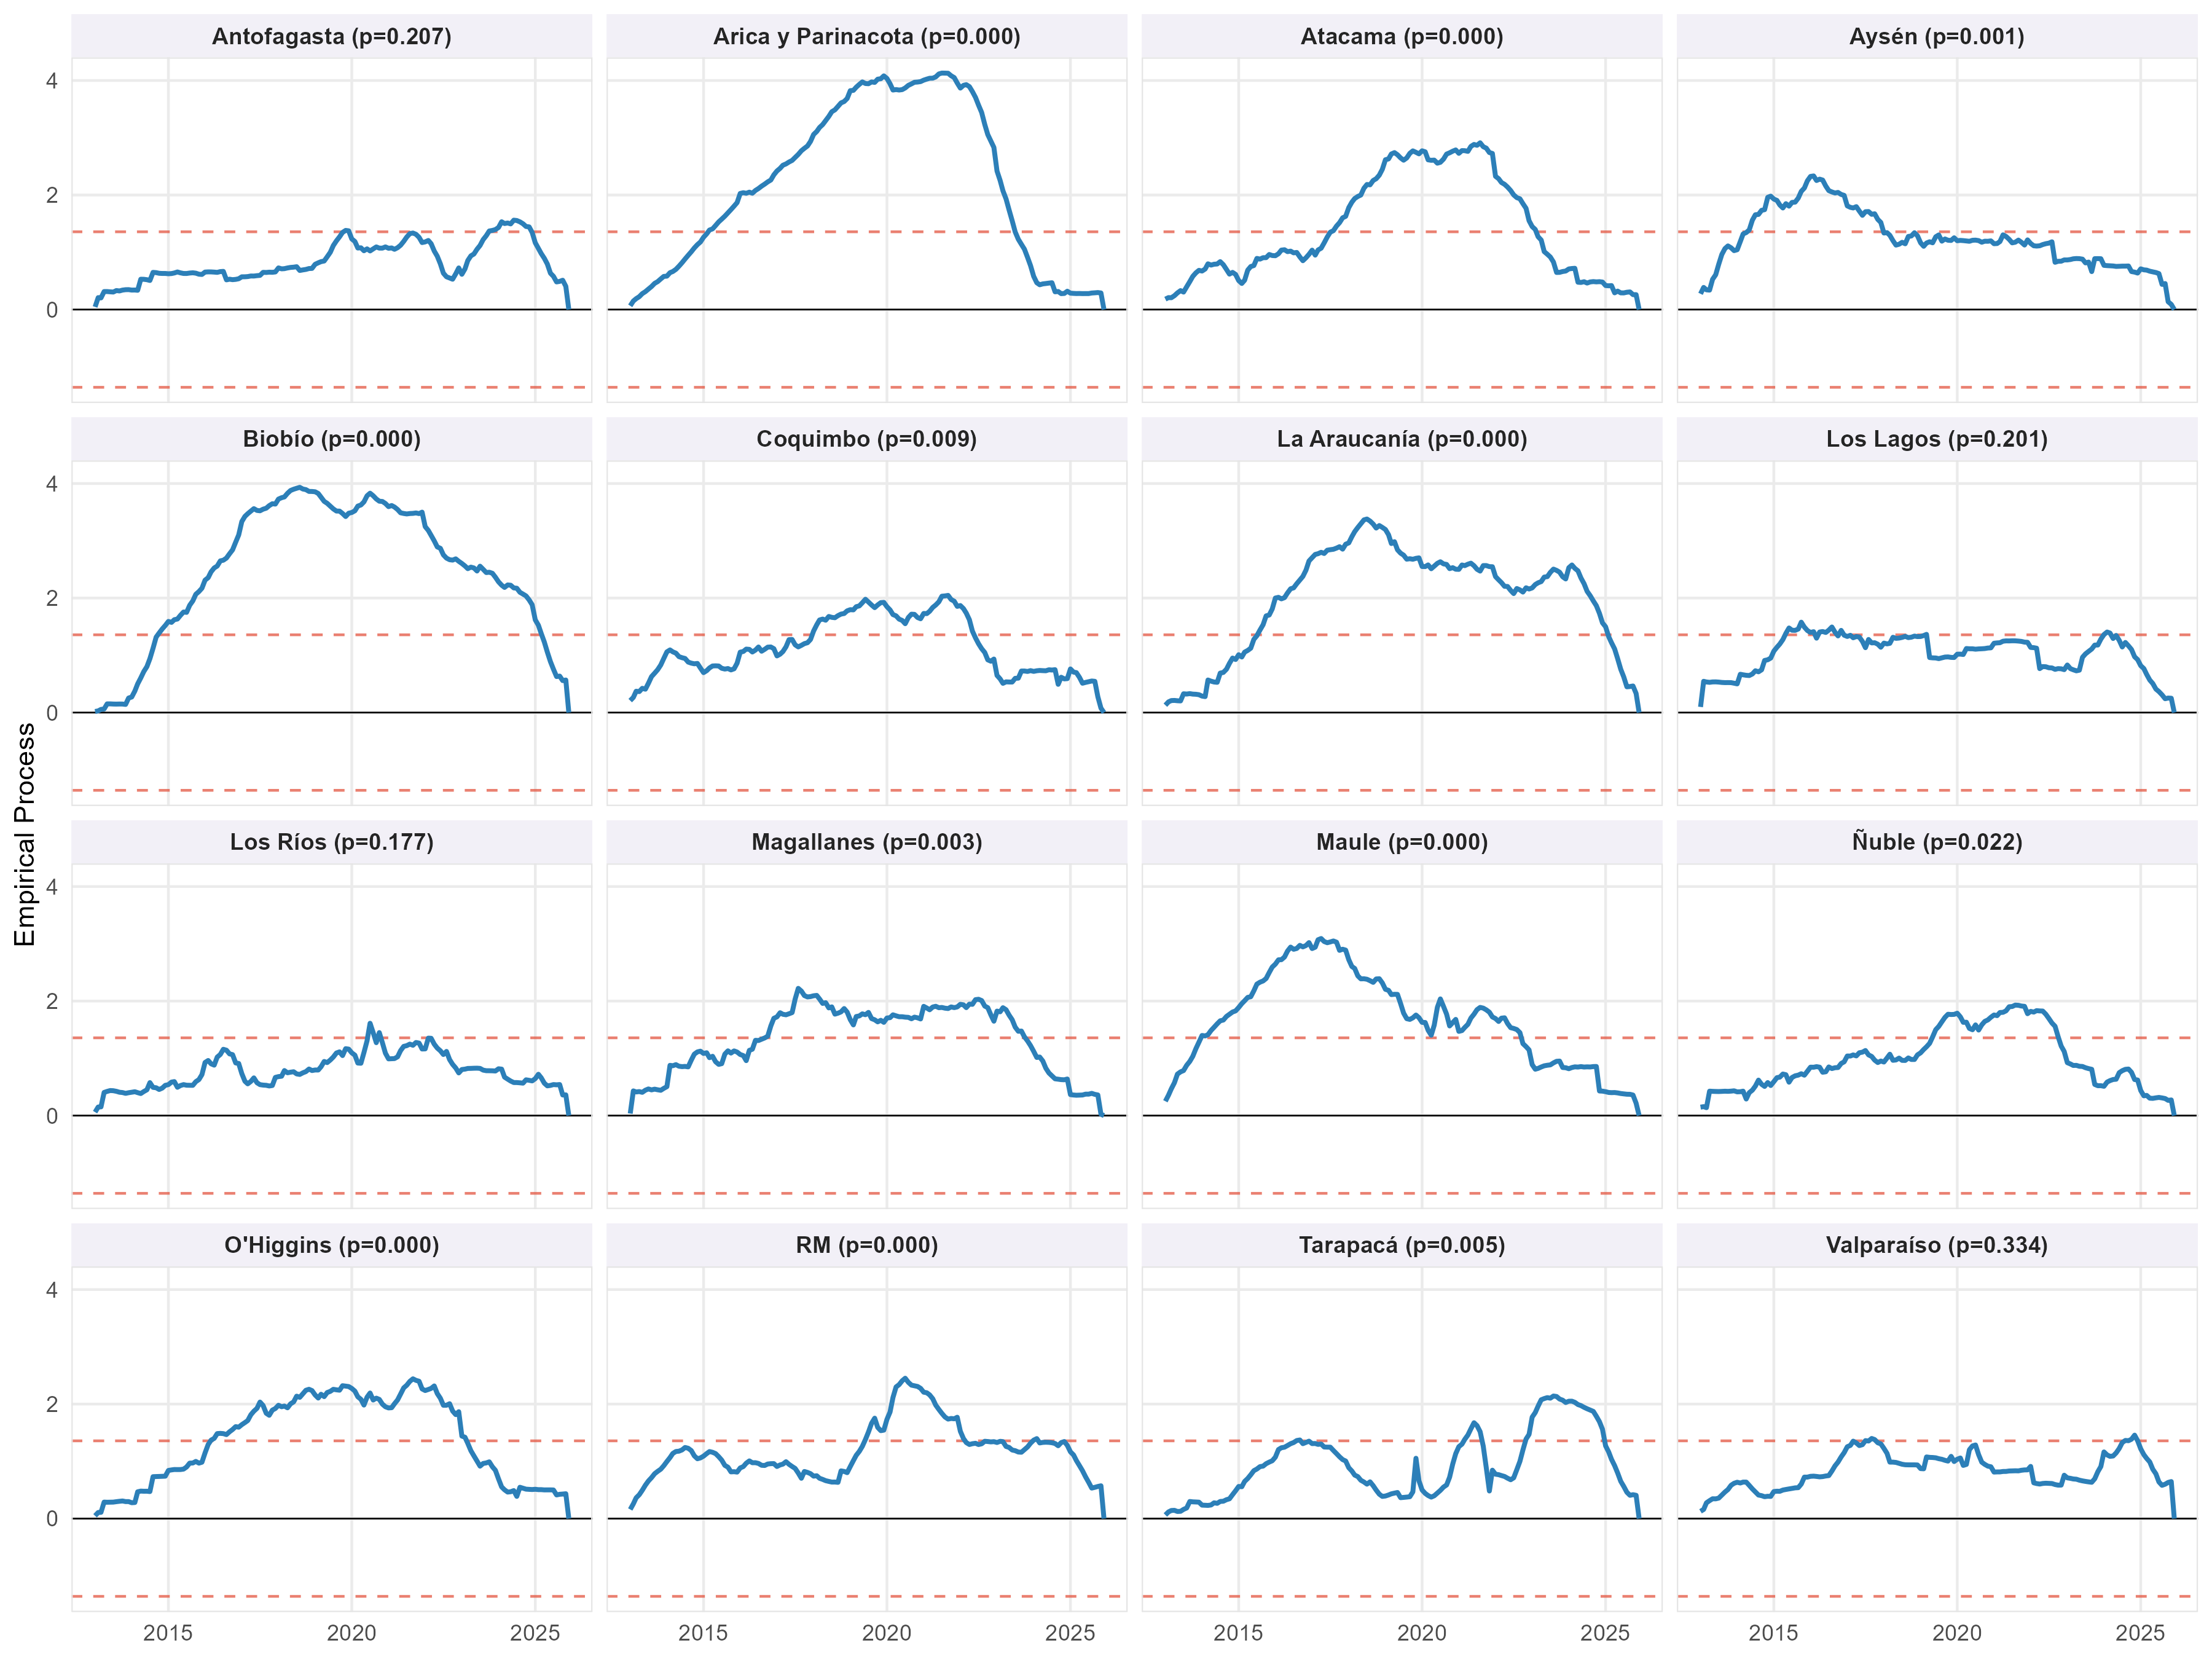
\includegraphics[width=\textwidth]{Fig4.png}
\caption{CUSUM-GLM processes for the 16 regions (confrontational robberies, C3.1).}
\label{fig:cusum}
\tablenote{The bands correspond to the 95\% critical limits of the Brownian bridge process. Regions with a significant break ($p$-FDR\,$<$\,0.05) are highlighted in red. Source: \citet{INE2026}; SERMIG; INE Base 2017 projections.}
\end{figure}

The macro-zone $\times$ spline interaction model (Appendix~\ref{ap:macro}) reveals that the long-term trend differs significantly across geographic zones (joint Wald test: $p<0.001$). In the first segment (Spline 1, 2013--2016), the Metropolitan Region exhibits the highest relative growth (IRR\,=\,2.68 compared to Austral), followed by the Central macro-zone (IRR\,=\,1.82). In Spline 2 (2016--2019), the North macro-zone leads with the highest IRR (3.94), consistent with accumulated migratory pressure and the CUSUM break identified in Arica y Parinacota. In Spline 3 (2019--2022), the Central zone reaches its highest dynamism (IRR\,=\,3.57). In Spline 4 (2022--2025), all macro-zone interactions converge substantially toward unity relative to Splines~2--3---North: IRR\,=\,1.08; Central: 1.37; RM: 1.46; South: 1.00---confirming that the recent downward inflection is a national-level phenomenon rather than an artifact of any particular zone.

\subsection{Falsification Tests}
\label{sub:placebos}

Four validation models provide convergent evidence regarding the specificity and power of the main model (Table~\ref{tab:placebos}).

The negative placebo (P1, vehicular accidents) reflects the post-pandemic reactivation of traffic activity: all its spline segments are positive and significant, with Spline 4 yielding an IRR\,=\,2.036 ($p<0.001$). The same model that detected a negative inflection in confrontational robberies captures a pronounced growth here. This rules out the possibility that the specification systematically underestimates activity in the recent period: the negative result for Spline 4 in confrontational robberies does not stem from model misspecification.

The positive placebo (P2, CCH homicides) offers a direct counter-test: if actual violence is increasing, the model must detect it. And it does.\footnote{CCH homicide complaints correspond to CUM~702 (\textit{homicidio simple}), CUM~703 (\textit{homicidio calificado}), and CUM~705 (\textit{parricidio}), restricted to formal citizen complaints (\textit{denuncias}); flagrant arrests are excluded.} Splines 2 and 3 record IRRs of 2.746 and 3.612 ($p<0.001$ in both), capturing the real increase in homicides between 2016 and 2022. For Spline 4, homicides yield an IRR\,=\,2.061 ($p<0.001$)---still indicating robust growth, contrasting sharply with the downward inflection seen in confrontational robberies. This divergence between homicides (growing in Spline 4) and confrontational robberies (decreasing) validates the model's discerning capability to trace opposing dynamics concurrently. Macro-zonal disaggregation reveals a key contrast.\footnote{These coefficients derive from separate Poisson-QMLE models estimated for each macro-zone by aggregating the regional panel, following the same specification as the main model.} The Northern macro-zone recorded an early, concentrated lethal surge during 2016--2019 (Spline 2: IRR\,=\,2.25, $p<0.001$) that attenuated in subsequent periods (Spline 3: IRR\,=\,1.66, $p=0.208$; Spline 4: IRR\,=\,0.89, $p=0.356$), indicating that lethal violence in that territory moderated following its early peak---consistent with the documented consolidation of organized crime routes in that border zone \citep{bravo2024}. By contrast, Central, RM, and Southern macro-zones exhibit prolonged and unresolved structural expansions: Spline~3 IRRs of 2.65, 2.89, and 2.85 respectively (all $p<0.05$), persisting into the most recent period with Spline~4 IRRs of 1.49, 1.56, and 1.68 (all $p\leq0.002$). The Austral macro-zone shows no significant trend in any segment. The juxtaposition of ongoing homicide growth in Central, RM, and South during 2022--2025 with the simultaneous moderation of confrontational robberies nationally confirms that the model tracks genuinely divergent dynamics: property crime violence is easing while lethal violence continues to escalate in most of the country.

A second positive placebo (P3, CCH reported kidnappings) provides complementary validation.\footnote{Kidnapping series covers CUM~202, 235, 236, 237, 248, and 249, comprising simple, extortionate, and aggravated kidnapping modalities, restricted to formal denuncias.} If coercive organized crime expanded between 2022--2025, the model should register kidnapping increments. Spline 4 for kidnappings yields an IRR\,=\,1.553 ($p<0.001$), the highest coefficient among the placebo specifications for the recent period, reinforcing the interpretation that organized coercive crime did expand. The coexistence of a downward inflection in aggregate confrontational robberies (IRR\,=\,0.868) alongside pronounced growth in kidnappings (IRR\,=\,1.553) confirms that the model accurately discriminates severity tiers: the drop in total volume does not preclude detecting highly injurious emerging phenomena.

Triangulating with confirmed CPHDV homicides provides the most robust benchmark against the dark figure. Annual records show growth from approximately 900 confirmed homicides in 2018 to a peak of 1,330 in 2022, followed by a sustained decrease: 1,249 in 2023, 1,209 in 2024, and 1,091 in 2025. The Spline 4 coefficient for CPHDV is not statistically significant (IRR\,=\,1.075, $p=0.530$), indicating that the growth of lethal violence decelerated recently. The parallel moderation between confirmed homicides and confrontational robberies sketches a coherent picture: both indicators point to a peak around 2022 and subsequent deceleration.

Two additional specifications---simple damage offenses (P4) and minor injury offenses (P5), estimated under the same model structure---are omitted from Table~\ref{tab:placebos} for parsimony but complete the analytical picture.\footnote{Simple damage offenses (P4): CUM~840 (\textit{da\~nos simples}). Minor injury offenses (P5): CUM~13001 (\textit{lesiones leves}). Vehicular accident placebo (P1): CUM~14020 (\textit{cuasidelito vehicular}). All placebo series are restricted to formal denuncias; flagrant arrests are excluded.} Simple damages declined consistently across all spline segments, with a Spline~4 IRR of 0.805 ($p<0.001$). Minor injuries followed an analogous trajectory (Spline~4: IRR\,=\,0.698, $p<0.001$). Together with the C3 categories and the four specifications in Table~\ref{tab:placebos}, these results establish a coherent severity gradient across the 2022--2025 period. The Spline~4 trend rises monotonically with offense severity: strong decline at the lowest tier---non-confrontational property offenses (IRR\,=\,0.648), minor injuries (0.698), simple damages (0.805)---through marginal decline at intermediate severity---snatching (0.861, n.s.) and confrontational robberies (0.868, $p=0.057$)---to strong growth at the highest coercive tier---kidnappings (1.553) and CCH homicides (2.061). This monotonic gradient---formalized as Table~\ref{tab:gradiente} in Section~\ref{sec:discusion}---is a direct empirical expression of the compositional shift described in Section~\ref{sec:marco}: as opportunity-dependent crimes contract, coercive and lethal modalities maintain or intensify their trajectory.

\begin{table}[htbp]
\centering
\caption{Placebos and external validation: Poisson-QMLE models}
\label{tab:placebos}
\footnotesize
\resizebox{\textwidth}{!}{
\begin{tabular}{l@{\hskip 3mm}ccc@{\hskip 4mm}cc@{\hskip 4mm}cc@{\hskip 4mm}cc}
\toprule
 & \multicolumn{3}{c}{\textbf{P1: Vehicular accident}} & \multicolumn{2}{c}{\textbf{P2: CCH Homicides}} & \multicolumn{2}{c}{\textbf{P3: Kidnappings}} & \multicolumn{2}{c}{\textbf{CPHDV (confirmed)}} \\
\cmidrule(lr){2-4}\cmidrule(lr){5-6}\cmidrule(lr){7-8}\cmidrule(lr){9-10}
\textbf{Term} & IRR & 95\% CI & $p$ & IRR & $p$ & IRR & $p$ & IRR & $p$ \\
\midrule
$D^{\text{est}}$ & 1.105 & [0.989, 1.234] & .078 & 1.144 & .097 & 0.869 & .146 & 1.046 & .763 \\
$D^{\text{pan}}$ & 0.874 & [0.750, 1.020] & .087 & 1.009 & .949 & 0.572 & $<$.001 & 0.871 & .367 \\
\midrule
Spline 1 &  9.080 & [3.09, 26.70] & $<$.001 & 1.300 & .096 & 1.338 & .024 & 1.562 & .001 \\
Spline 2 &  3.820 & [1.85,  7.90] & $<$.001 & 2.746 & $<$.001 & 2.654 & $<$.001 & 1.430 & $<$.001 \\
Spline 3 & 48.380 & [6.78, 345.4] & $<$.001 & 3.612 & $<$.001 & 1.649 & .024 & 1.774 & .113 \\
\textbf{Spline 4} & \textbf{2.036} & \textbf{[1.397, 2.969]} & \textbf{$<$.001} & \textbf{2.061} & \textbf{$<$.001} & \textbf{1.553} & \textbf{$<$.001} & 1.075 & .530 \\
\bottomrule
\end{tabular}
}
\tablenote{P1, P2, and P3 are estimated over the regional panel (16 regions $\times$ 156 months); CPHDV on a national series (2018--2025, independent knots). The large IRRs for P1 in Spline 3 reflect post-pandemic traffic normalization on a logarithmic scale. Inference: WCB (Webb weights, $B=9,999$) for P1, P2, and P3; standard QMLE errors for CPHDV.}
\end{table}

% =========================================================
\section{Robustness Checks}
\label{sec:robustez}
% =========================================================

The primary finding---the downward inflection of Spline 4 for confrontational robberies (IRR\,=\,0.868, $p=0.057$)---is verified across five specification variants addressing four uncertainty dimensions.

The first dimension addresses the demographic denominator. Specification R1 replaces the fixed offset with the logarithm of the population as a regressor, relaxing the exact proportionality assumption; R2 drops the SERMIG migratory correction entirely, anchoring the denominator strictly upon pre-existing INE projections without migratory updates. R1 confirms and strengthens the principal result (IRR\,=\,0.732, $p=0.010$). R2 constitutes the sole exception among the five specifications, producing a practically null coefficient (IRR\,=\,0.994, $p=0.948$): omitting migratory flows from the denominator introduces noise in high-immigration regions, attenuating the signal toward zero. This result does not contradict the direction of the main finding; rather, it highlights the empirical relevance of the SERMIG correction as a necessary methodological component.

The second dimension evaluates whether the results depend on the spline knot parameterization. In R3, the knots are fixed at four historical-political dates relevant to the period: April 2014 (start of Michelle Bachelet's second term), April 2018 (start of Sebasti\'an Pi\~nera's second term), November 2019 (social uprising), and October 2021 (end of the post-pandemic state of constitutional exception). With these four knots, the spline generates five trend segments; the last one---November 2021 to December 2025---is the relevant segment for comparison. R3 produces an IRR of 0.899 ($p=0.118$): directly consistent in sign with the main result although without reaching conventional statistical significance. Directional replication with theoretically predefined knots confirms the downward inflection is not an artifact of the empirical knot locations.

The third dimension concerns the dependent variable. R4 replaces citizen reports with flagrancy arrests, which are police-initiated and structurally independent of the citizen propensity to report. Under a pure reporting-artifact hypothesis---in which the decline in reports reflects fewer citizens filing complaints rather than fewer crimes---arrests should remain stable or diverge from reports. R4 yields an IRR\,=\,0.539 ($p<0.001$), confirming the directional finding in the enforcement-detected series: flagrancy arrests moved in the same direction as reports during 2022--2025. The larger magnitude relative to the main model warrants interpretation, however. The gap between 0.539 and 0.868 need not imply that arrests \emph{overestimate} the decline in crime; it may equally reflect a concurrent reduction in police proactive patrol capacity or a strategic reallocation of enforcement resources away from confrontational property offense in recent years---a supply-side factor that operates orthogonally to actual crime volume. R4 should therefore be read as directional confirmation of the downward inflection rather than as a precise counterfactual estimate of its magnitude.

The fourth dimension increases the functional flexibility of the spline. R5 increases the degrees of freedom from four to five, allowing a more flexible functional form. R5 replicates the magnitude of the principal result almost identically (IRR\,=\,0.863, $p=0.068$), confirming that the inflection is insensitive to the number of spline terms. Ultimately, four out of the five alternative specifications return negative evaluations yielding IRRs spanning 0.539 to 0.899. The alternative binary classifications C1 and C2 (Appendix~\ref{ap:clasif}) constitute a fifth robustness layer: C2 fully replicates the C3.1 results (IRR\,=\,0.868, $p=0.057$), while C1 substantially attenuates the estimates by merging snatching into the violent category. Table~\ref{tab:robustez} reports the Spline~4 coefficients across all specifications for confrontational robberies.

\begin{table}[htbp]
\centering
\caption{Robustness analysis: trend coefficient beneath alternate equivalents (confrontational robberies, C3.1)}
\label{tab:robustez}
\footnotesize
\resizebox{\textwidth}{!}{
\begin{tabular}{llccc}
\toprule
\textbf{ID} & \textbf{Specification} & \textbf{Estimator}\textsuperscript{a} & \textbf{IRR} & $p$ \\
\midrule
Main & Base model (spline P25/P50/P75, WCB) & $-$0.141 & 0.868 & .057 \\
\midrule
R1 & Free offset (pop. as regressor)    & $-$0.312 & 0.732 & .010 \\
R2 & Without SERMIG correction               & $-$0.006 & 0.994 & .948 \\
R3 & Historical-political knots (2014, 2018, 2019, 2021) & $-$0.107 & 0.899 & .118 \\
R4 & Arrests as dependent variable & $-$0.618 & 0.539 & $<$.001 \\
R5 & More flexible spline (df\,=\,5)      & $-$0.147 & 0.863 & .068 \\
\bottomrule
\end{tabular}
}
\tablenote{\textsuperscript{a} The reported estimator corresponds to Spline~4 of the model (trend in the 2022--2025 period). All specifications include uprising/pandemic dummies, regional fixed effects, and monthly seasonality.}
\end{table}

Table~\ref{tab:sensipop} examines sensitivity to the irregular population denominator under demographic inflation factors $k \in \{1.00, 1.05, 1.10, 1.15, 1.20\}$ applied to high-immigration regions. Point estimates are perfectly stable across all iterations (IRR\,=\,0.868), with $p$-values ranging narrowly from 0.048 to 0.062. This invariance arises because the inflation factor $k$ rescales the population offset additively on the log scale, shifting the intercept while leaving the trend slope unaffected. The results are therefore robust to any plausible assumption about irregular populations not captured by SERMIG.

\begin{table}[htbp]
\centering
\caption{Sensitivity to irregular denominator: inflation factor $k$ on corrected population (confrontational robberies)}
\label{tab:sensipop}
\footnotesize
\begin{tabular}{ccccc}
\toprule
\textbf{Factor $k$}\textsuperscript{a} & \textbf{Estimator} & \textbf{SE (WCB)} & \textbf{IRR} & $p$ \\
\midrule
1.00 & $-$0.141 & 0.071 & 0.868 & .048 \\
1.05 & $-$0.141 & 0.075 & 0.868 & .061 \\
1.10 & $-$0.141 & 0.074 & 0.868 & .057 \\
1.15 & $-$0.141 & 0.072 & 0.868 & .050 \\
1.20 & $-$0.141 & 0.076 & 0.868 & .062 \\
\bottomrule
\end{tabular}
\tablenote{\textsuperscript{a} $k$ = inflation factor applied to the corrected population of high-immigration regions (Tarapac\'a, Antofagasta, Arica y Parinacota, Metropolitan Region). Invariance confirms that trend estimates are unaffected by assumptions about irregular populations not captured by SERMIG.}
\end{table}

% =========================================================
\section{Discussion}
\label{sec:discusion}
% =========================================================

The empirical evidence presented here revises the dominant diagnosis surrounding property crime in Chile: the main pattern is not a generalized volumetric crisis in reported robbery and theft, but a compositional transformation within reported physical property crime. The ratio of confrontational robberies to (confrontational~$+$~non-confrontational) property offenses reached a historical peak of 21.6\% in January 2024, traced across four successive Bai-Perron breaks; however, its driving mechanism is not an increase in confrontational robberies, but the more pronounced and structural decline of non-confrontational property offenses (Spline 4: IRR\,=\,0.648, $p<0.001$, a 35.2\% reduction against the initial level). The two types comprising 93\% of the group---intimidation and direct violence---display post-pandemic frequencies beneath their historical 2016--2019 reference thresholds. The statistical paradox---an escalating ratio alongside a stabilized or downward-inflecting volume---is arithmetically driven by two structural forces: the pronounced contraction of contactless theft opportunities and the comparatively greater resistance of coercive crime to those same barriers. A third parallel development---the emergence of robbery with victim retention or severe injuries---reinforces the direction of the compositional shift without constituting a primary driver of the ratio, given its currently marginal share of the confrontational robbery cluster ($<$0.1\%).

The two shocks during the period are not merely statistical controls; their differential effects across crime types are consistent with the theoretical mechanisms proposed in Section~\ref{sec:marco}, though the study's observational design does not permit ruling out alternative explanations. During the social uprising, coercive crime rose sharply (confrontational robberies: IRR\,=\,1.155, $p<0.001$)---a pattern theoretically interpretable under institutional delegitimization mechanisms \citep{tyler2006,rosenfeld2021}---while snatching also increased (IRR\,=\,1.069, $p<0.001$), suggestive of amplified snatching opportunity during the massive occupation of public spaces, consistent with routine activity theory \citep{cohen1979}. Structural property crime lacking victim contact remained unaffected (non-confrontational: IRR\,=\,0.996, $p=0.761$), a pattern consistent with---though not confirming---the hypothesis that demand-driven offenses respond primarily to ambient opportunity structures rather than social conflict dynamics. This three-way differential---coercive rising, agglomeration-sensitive rising, contactless flat---is a direct empirical output of the trichotomous classification and would be invisible under binary aggregation. By contrast, the pandemic contracted all crime types broadly in proportion to their agglomeration dependence (snatching: $-$42.4\%; non-confrontational: $-$35.3\%; confrontational: $-$34.9\%): snatching collapsed most sharply, a pattern consistent with their documented sensitivity to pedestrian agglomeration and mass transit use, while confrontational and non-confrontational categories contracted to a nearly indistinguishable degree---broadly consistent with the predictions of routine activity theory \citep{cohen1979,ashby2020,stickle2020} and the economic perspective that mobility restrictions raise the opportunity costs of agglomeration-dependent crimes differentially \citep{becker1968}. These patterns align with comparative evidence on mass protests \citep{bell2014,mongale2022} and pandemic impacts on crime \citep{ashby2020,stickle2020}.

The post-pandemic trajectory replicates the pattern that \citet{blumstein1988} identified in sustained crime declines: high-severity offenses exhibit greater downward resistance than opportunistic ones. Non-confrontational property offenses did not recover after mobility normalized; their structural decline---consistent with permanent shifts in post-COVID routines such as the persistence of remote work \citep{seyidoglu2024}, e-commerce expansion, and enhanced residential security, though causal attribution to any single factor is beyond this study's scope---absorbed and surpassed any rebound component, deepening monotonically across all four spline segments (IRR = 0.718, 0.685, 0.656, 0.648). Confrontational robberies, on the other hand, recovered their baseline level in 2022--2023 and initiated a downward inflection confirmed in Spline~4 (IRR\,=\,0.868, $p=0.057$), suggestive though at the edge of conventional significance with $G=16$ clusters. This downward inflection is temporally consistent with the policy environment of the period: public security expenditure---which contracted to 1.4\% of GDP in 2022 following the pandemic---was gradually recovered by the Boric administration to 1.5\% of GDP by early 2024, rising from a trough of 3.9\% to 5.8\% as a share of central government spending \citep{dominguez2023gasto}; this budgetary effort continued into 2025, with allocations explicitly targeting organized crime under the government's prioritization of citizen security as the country's primary public concern \citep{diaz2024presupuesto}. Causal attribution from observational data remains beyond the scope of this study, but the temporal alignment between sustained institutional investment and the observed moderation in coercive robbery rates is suggestive that policy capacity may have contributed to the inflection. The growing ratio is the arithmetic residue of unequal decline velocities: crimes executable with lower risk contract faster than those requiring direct victim confrontation.

Table~\ref{tab:gradiente} formalizes the severity gradient identified in Section~\ref{sub:placebos}. The perfectly monotonic sequence---0.648, 0.698, 0.805, 0.861, 0.868, 1.553, 2.061---across seven specifications estimated under identical model structure is consistent with two complementary theoretical mechanisms, though the observational design of this study cannot establish these mechanisms as causal. Under \citet{becker1968}'s rational model, crimes differ in their ``production function'': contactless theft operates under low execution costs but is highly sensitive to any factor that raises opportunity barriers---payment digitization, residential security investment, reduced pedestrian density---because the offender depends on passive opportunity. Crimes requiring direct coercive confrontation face a qualitatively different calculus: the offender manufactures the encounter rather than waiting for it, replacing ambient opportunity with deliberate target selection. Under this framework, each step up the severity ladder corresponds to lower opportunity-elasticity; structural contraction would therefore produce a gradient that is monotonically less negative (or more positive), as observed. \citet{cohen1979}'s routine activity theory reaches an equivalent prediction from a convergence logic: contactless crime requires the simultaneous convergence of a motivated offender, a suitable target, and an absent guardian in time and space. Structural shifts---remote work, e-commerce normalization, residential security investment---may systematically disrupt this convergence for opportunity-dependent modalities. Confrontational robbery, in contrast, is offender-initiated: the convergence is manufactured, not awaited, rendering it potentially less sensitive to ambient guardianship conditions. At the extreme end of the gradient, kidnappings and homicides are consistent with an organizational rather than opportunistic rationale---operations potentially driven by networks with embedded enforcement capacity \citep{dammert2025,greene2023}---which would make them structurally decoupled from the environmental factors suppressing contactless crime \citep[see also][for evidence of crime persistence via lagged effects across offense types]{buonanno2008}. The seven-point monotonic gradient is interpretable as the aggregate empirical signature of these micro-level asymmetries, though multiple mechanisms could produce the same pattern.

\begin{table}[htbp]
\centering
\caption{Severity gradient: Spline~4 (October 2022--December 2025) IRR across all specifications, ordered by offense severity}
\label{tab:gradiente}
\footnotesize
\begin{tabular}{lllcc}
\toprule
\textbf{Offense / Category} & \textbf{Source} & \textbf{Spline 4 IRR} & \textbf{95\% CI} & $p$ \\
\midrule
\multicolumn{5}{l}{\textit{Declining trend}} \\
Non-confrontational property offenses (C3.3) & Main model & 0.648 & [0.580, 0.723] & $<$.001 \\
Minor injuries (P5)          & Placebo    & 0.698 & ---\textsuperscript{a}            & $<$.001 \\
Simple damages (P4)          & Placebo    & 0.805 & ---\textsuperscript{a}            & $<$.001 \\
Snatching (C3.2)    & Main model & 0.861 & [0.511, 1.450] & .574 \\
Confrontational robberies (C3.1)     & Main model & 0.868 & [0.751, 1.004] & .057 \\
\midrule
\multicolumn{5}{l}{\textit{Increasing trend}} \\
Kidnappings (P3)             & Placebo    & 1.553 & ---\textsuperscript{a}            & $<$.001 \\
CCH Homicides (P2)           & Placebo    & 2.061 & ---\textsuperscript{a}            & $<$.001 \\
\bottomrule
\end{tabular}
\tablenote{All specifications use the same Poisson-QMLE structure (balanced region-month panel, 16 regions $\times$ 156 months) with regional fixed effects, monthly seasonality dummies, social uprising/pandemic controls, and Wild Cluster Bootstrap inference. \textsuperscript{a} CIs omitted for parsimony; see Table~\ref{tab:placebos}. The seven values form a perfectly monotonic sequence from 0.648 to 2.061. The ordering reflects a dimension running from maximum ambient-opportunity dependence (non-confrontational property offenses, minor injuries, simple damages) through offender-initiated confrontation (surprise and confrontational robberies) to organizational enforcement capacity (kidnappings, homicides). Minor injuries (0.698) decline faster than simple damages (0.805) not because they are less coercive---street altercations involve victim contact while vandalism often does not---but because they are more agglomeration-dependent.}
\end{table}

The territorial dimension reveals that beneath the national aggregate operate qualitatively distinct local dynamics. This finding resonates with evidence from \citet{campedelli2020}, who demonstrated that aggregate city-level crime trends during COVID-19 lockdowns in Chicago concealed substantial community-level heterogeneity---with significant reductions observed in only a subset of neighborhoods, moderated by population density and socioeconomic conditions---underscoring the analytical cost of treating jurisdictions as internally homogeneous units. The three groups of regional breaks identified by the CUSUM tests do not represent variants of a single phenomenon: each reflects its own underlying logic. The pre-pandemic breaks in the south (Araucan\'ia: July 2018; Biob\'io: August 2018) precede the social uprising by over a year and reflect the escalation of the local territorial conflict \citep{izquierdo2024}, not a national shock. In the Northern macro-zone, confrontational robbery breaks occurred between 2021 and 2023, following the lethal violence surge of that territory during 2016--2019 (homicide Spline 2 in North: IRR\,=\,2.25, $p<0.001$; see Section~\ref{sub:placebos}) and consistent with the subsequent stabilization of lethal violence in that territory (homicide Spline 4: IRR\,=\,0.89, $p=0.356$). This temporal dissociation aligns with the hypothesis of a growing presence of organized modalities in the area, although this article's evidence cannot establish causality in that direction \citep{bravo2024,crespo2023}. By contrast, Central, RM, and Southern macro-zones continue to record significant homicide growth in Spline 4 (IRRs of 1.49, 1.56, and 1.68; all $p\leq0.002$), reinforcing the finding that lethal violence has not moderated in most of the country even as aggregate confrontational robbery rates begin to ease. The convergence of confrontational robbery macro-zone IRRs toward unity in Spline 4 confirms that the robbery inflection is a national phenomenon; the same convergence is absent for homicides, underscoring the qualitative distinction between the two dynamics.

Beneath the aggregate trend lies a signal demanding specific monitoring within the confrontational robberies group: robbery involving victim retention or severe injuries (CUM~862), whose average rate in 2022--2025 (0.878 per 100,000) is 263\% above the 2016--2019 baseline (0.242 per 100,000), with annual counts growing from 83 in 2022 to 283 in 2025. The magnitude partly reflects the low starting point---this crime represents less than 0.1\% of the total group---but the trend is sustained and the modality involves prolonged coercion or direct violence against the victim, qualitatively distinguishing it from conventional property robbery and justifying differentiated monitoring. This signal is coherent with the P3 placebo result (CCH kidnappings: Spline 4 IRR\,=\,1.553, $p<0.001$): certain specific coercive modalities show expansion recently precisely as the aggregate volume of confrontational robberies moderates, illustrating why the volume vs composition distinction is not solely analytical, but politically urgent.

A complementary signal---operating outside the CCH property crime taxonomy but carrying structural implications for it---concerns the expansion of digital fraud. Administrative records for fraud against private individuals and fraudulent use of payment instruments\footnote{The four administrative codes evaluated are: CUM~816 (\textit{Estafas y otras defraudaciones contra particulares}), covering fraud and other deception offenses under Arts.~467--470 and 473 of the Penal Code; CUM~12151 (\textit{Uso fraudulento de tarjetas o medios de pago}), covering fraudulent use of credit cards, debit cards, or prepaid payment instruments subject to CMF and Central Bank of Chile regulation; CUM~12201 (\textit{Uso malicioso de tarjeta, clave o dispositivo financiero}) and CUM~12202 (\textit{Obtención maliciosa o restitución de fondos de operaciones reclamadas}), both introduced in 2024 as an administrative disaggregation of CUM~12151 under Art.~7(a) of Law~20.009, which sanctions the malicious use of blocked payment instruments and the fraudulent obtainment of fund reversals through false declarations or simulated unauthorized transactions.} exhibit a trajectory that mirrors, in reverse, the secular decline of physical non-confrontational property offenses: from approximately 9\% of non-confrontational property offense volume in 2013, digital fraud reached roughly 40\% in 2019, contracted during the pandemic, then surged to 72\% in 2024 and exceeded non-confrontational property offense volume entirely in 2025 (114\%). This trajectory cannot be analyzed within the CCH property crime framework applied here---the coding structures, reporting incentives, and criminological mechanisms of fraud are qualitatively distinct from those of contactless physical theft---but it raises a theoretically consequential question: does the secular decline in physical non-confrontational property crime partly reflect a \emph{modal substitution} toward technologically mediated property crime rather than genuine crime contraction? If victims of phone-based scams or payment card fraud are displacing victims of burglary or shoplifting within a shared pool of property victimization, the compositional shift described in this article extends beyond the violence/non-violence axis into a physical/digital axis, with far-reaching implications for measurement frameworks, victimization survey design, and theoretical models of property crime opportunity.

The distinction between volume and composition bears direct consequences for intervention design. A volumetric response---increased police presence aiming to reduce total incident count---misses the target when the underlying dynamic is compositional. It would predominantly reduce non-confrontational property offenses, which are already structurally declining, without addressing the most severe coercive phenomena. Effective interventions demand approaches differentiated by crime type and targeted toward the specific dynamics of each emerging modality.

Five limitations must be considered. The effect of the Virtual Police Station on reporting propensity cannot be directly controlled, although any such bias would operate against the main finding---inflating non-confrontational property crime records, not violent ones. Violent vehicle theft (CUM~867) records significant volume only since 2020, restricting the historical comparability of this segment within the confrontational robberies aggregate. The small number of clusters ($G=16$) suggests interpreting the confrontational robbery Spline 4 p-value ($p=0.057$) cautiously, although consistency across robust specifications, placebos, and descriptive analysis mitigates this constraint. The SERMIG correction provides a lower bound for actual population; the sensitivity analysis demonstrates coefficient invariance under multiple irregular population assumptions ($k \in \{1.00\text{--}1.20\}$). Finally, the analysis operates at the regional level, missing finer intra-regional heterogeneity that could be critical for local intervention design.

The future research agenda unfolds across four fronts. Offender profiling: reporting data cannot distinguish between serious individual-level crime and organized criminal structures; an analysis of the prosecution funnel---from complaint to conviction---could estimate this composition. Communal-level analysis: the 346 municipalities offer sufficient variance to determine whether the compositional shift is homogeneous within regions or responds to tighter urban concentrations. Monitoring emerging signals: determining whether the Spline 4 downward inflection consolidates past 2025, or whether victim retention escalates into an extortionary modality carrying greater statistical weight, are questions only systematic monitoring can answer. Physical-to-digital substitution: whether the structural decline of non-confrontational physical property offenses reflects genuine crime suppression or a displacement toward technologically mediated property crime warrants investigation combining victimization survey data---which can capture digital fraud alongside traditional robbery---with interrupted time series methods sensitive to the administrative discontinuities that complicate direct comparison of physical and digital offense series.

% =========================================================
\section{Conclusions}
\label{sec:conclusiones}
% =========================================================

This article evaluated whether Chile faces a volumetric crisis in reported confrontational robbery or a compositional shift in reported physical property crime. The results are unequivocal in one direction and provisional in another. Unequivocally: the two categories grouping 93\% of confrontational robberies---intimidation and direct violence---record post-pandemic rates below their historical baseline (2016--2019), and non-confrontational property offenses exhibit a robust secular decline reaching a 35.2\% reduction in the most recent period (Spline 4: IRR\,=\,0.648, $p<0.001$). The ratio of confrontational robberies to (confrontational~$+$~non-confrontational) property offenses hit its historical peak of 21.6\% in January 2024, propelled not by a surging numerator but by the steeper drop of non-confrontational offenses in the denominator. This paradox---growing ratio, stabilized or downward-inflecting volume---is the central finding: the debate over the ``crisis'' captures something qualitatively real, but overestimates the phenomenon by conflating volume with composition. Provisionally: the downward inflection of Spline 4 in confrontational robberies (IRR\,=\,0.868, $p=0.057$) is suggestive but sits at the threshold of conventional significance with $G=16$ clusters; its consolidation will depend on data from subsequent years.

The two shocks of the period empirically validate the theoretical framework. The social uprising was associated with increases in both coercive crime (confrontational robberies: IRR\,=\,1.155, $p<0.001$), consistent with institutional delegitimization dynamics \citep{tyler2006,rosenfeld2021}, and snatching (IRR\,=\,1.069, $p<0.001$), consistent with crowd-driven opportunity amplification \citep{cohen1979}, while leaving structural property crime unaltered (non-confrontational: IRR\,=\,0.996, $p=0.761$)---a three-way differential interpretable under, though not directly proving, the trichotomous classification's theoretical logic. The pandemic suppressed all types, most sharply for snatching---a pattern consistent with their documented sensitivity to pedestrian agglomeration---while confrontational and non-confrontational categories contracted to a nearly indistinguishable degree (snatching: $-$42.4\%; non-confrontational: $-$35.3\%; confrontational: $-$34.9\%), broadly consistent with the predictions of routine activity theory \citep{cohen1979} and the economic perspective \citep{becker1968}. Placebos confirm the model's discriminating capability: vehicular accidents show the opposite behavior in Spline 4 (IRR\,=\,2.036, $p<0.001$), eliminating model misspecification as the source of the inflection. The territorial dimension reveals heterogeneous local dynamics beneath the national trajectory: pre-pandemic breaks in the south (CUSUM, 2017--2018), delayed breaks in the north (Tarapac\'a: August 2023) consistent with migratory pressures and border organized crime \citep{bravo2024,crespo2023}, and a convergence of all macro-zones toward unity in Spline 4, confirming that the recent downward inflection constitutes a national-scope phenomenon.

The methodological contribution is threefold: a 156-month panel series featuring migratory demographic correction, the trichotomous C3 classification exposing heterogeneity masked by binary structures, and the Poisson-QMLE strategy complemented by Wild Cluster Bootstrap inference, CUSUM-GLM modeling, and CPHDV triangulation. Beneath the primary result emerges a signal demanding individualized monitoring: robbery with victim retention or severe injury (CUM~862) logged zero reports between 2013 and 2016, surfaced in 2017 with 40 cases, grew to 83 in 2022, and reached 283 in 2025. Although it comprises less than 0.1\% of the confrontational robbery cluster, the trend proves persistent, and the modality---imposing prolonged coercion or direct violence against victims---is qualitatively distinct from conventional property robbery. Addressing a compositional change with interventions engineered for volumetric surges will fall short: public policy must focus fundamentally on high-severity emergent phenomena hidden within aggregate counts instead of targeting the counts that obscure them.

% =========================================================
%  REFERENCES
% =========================================================
\renewcommand{\refname}{References}
\begin{thebibliography}{51}
\providecommand{\natexlab}[1]{#1}
\providecommand{\url}[1]{{#1}}
\providecommand{\urlprefix}{URL }
\providecommand{\doi}[1]{\url{https://doi.org/#1}}
\providecommand{\eprint}[2][]{\url{#2}}
 \bibcommenthead

\bibitem[{Ashby(2020)}]{ashby2020}
Ashby MP (2020) Initial evidence on the relationship between the coronavirus
  pandemic and crime in the {United States}. Crime Science 9(1):6.
  \doi{10.1186/s40163-020-00117-6}

\bibitem[{Bai and Perron(1998)}]{bai1998}
Bai J, Perron P (1998) Estimating and testing linear models with multiple
  structural changes. Econometrica 66(1):47--78

\bibitem[{Becker(1968)}]{becker1968}
Becker GS (1968) Crime and punishment: {A}n economic approach. Journal of
  Political Economy 76:169--217. \doi{10.1086/259394}

\bibitem[{Bell et~al.(2014)Bell, Jaitman, and Machin}]{bell2014}
Bell B, Jaitman L, Machin S (2014) Crime deterrence: {E}vidence from the
  {London} 2011 riots. The Economic Journal 124(576):480--506.
  \doi{10.1111/ecoj.12137}

\bibitem[{Bisca et~al.(2024)Bisca, Chau, Dudine, Espinoza, Fournier, Guerin,
  Hansen, and Salas}]{bisca2024}
Bisca PM, Chau V, Dudine P, et~al (2024) Violent crime and insecurity in {Latin
  America} and the {Caribbean}. Departmental Papers~1, International Monetary
  Fund, \doi{10.5089/9798400288470.087}

\bibitem[{Blumstein et~al.(1988)Blumstein, Cohen, Roth, and
  Visher}]{blumstein1988}
Blumstein A, Cohen J, Roth JA, et~al (eds)  (1988) Criminal Careers and
  ``{Career Criminals}''. National Academy Press, Washington, D.C.

\bibitem[{Bowman et~al.(2024)Bowman, Kramer, Salau, and
  Matzopoulos}]{bowman2024}
Bowman B, Kramer S, Salau S, et~al (2024) Trends, correlates, and contexts of
  robbery-homicide in {South Africa}. Homicide Studies 28(1):27--51.
  \doi{10.1177/1088767921107023}

\bibitem[{Brantingham and Brantingham(1984)}]{brantingham1984}
Brantingham PJ, Brantingham PL (1984) Patterns in Crime. Macmillan, New York

\bibitem[{Bravo(2024)}]{bravo2024}
Bravo G (2024) Migraciones, narcotr\'afico y frontera. {L}a situaci\'on en la
  macrozona norte de {Chile}. 2020--2022. Di\'alogo Andino (73):128--140.
  \doi{10.4067/S0719-26812024000100128}

\bibitem[{Buonanno and Montolio(2008)}]{buonanno2008}
Buonanno P, Montolio D (2008) Identifying the socio-economic and demographic
  determinants of crime across {Spanish} provinces. International Review of Law
  and Economics 28(2):89--97. \doi{10.1016/j.irle.2008.02.005}

\bibitem[{Cameron and Miller(2015)}]{cameron2015}
Cameron AC, Miller DL (2015) A practitioner's guide to cluster-robust
  inference. Journal of Human Resources 50(2):317--372

\bibitem[{Campedelli et~al.(2020)Campedelli, Favarin, Aziani, and
  Piquero}]{campedelli2020}
Campedelli GM, Favarin S, Aziani A, et~al (2020) Disentangling community-level
  changes in crime trends during the {COVID-19} pandemic in {Chicago}. Crime
  Science 9(1):21. \doi{10.1186/s40163-020-00131-8}

\bibitem[{{Centro de Estudios P\'ublicos}(2025)}]{cep2025}
{Centro de Estudios P\'ublicos} (2025) Encuesta {CEP} {N}$^\circ$94 mayo--junio
  2025: {ISSP} orientaciones laborales. Tech. rep., Centro de Estudios
  P\'ublicos, Santiago, Chile,
  \urlprefix\url{https://www.cepchile.cl/encuesta/encuesta-cep-n-94-mayo-junio-2025-issp-orientaciones-laborales/}

\bibitem[{Clarke(1995)}]{clarke1995}
Clarke RV (1995) Situational crime prevention. In: Tonry M, Farrington DP (eds)
  Building a Safer Society: Strategic Approaches to Crime Prevention, Crime and
  Justice, vol~19. University of Chicago Press, Chicago, p 91--150

\bibitem[{Cohen and Felson(1979)}]{cohen1979}
Cohen LE, Felson M (1979) Social change and crime rate trends: {A} routine
  activity approach. American Sociological Review 44(4):588--608.
  \doi{10.2307/2094589}

\bibitem[{Crespo and Lay(2023)}]{crespo2023}
Crespo F, Lay C (2023) Una d\'ecada en {Chile}: {A}n\'alisis de homicidios,
  abusos sexuales y robos con intimidaci\'on desde 2010 a 2022. Observatorio
  Econ\'omico (184):5--13. \doi{10.11565/oe.v1i184.535}

\bibitem[{Dammert et~al.(2025)Dammert, Frey, and Gonz\'alez}]{dammert2025}
Dammert L, Frey A, Gonz\'alez P (2025) Concentraci\'on territorial de
  homicidios, secuestros y extorsiones: {E}l caso de la {Regi\'on
  Metropolitana} de {Santiago de Chile}. Pol\'itica Criminal 20(40):269--294.
  \doi{10.4067/s0718-33992025000200269}

\bibitem[{D\'iaz(2024)}]{diaz2024presupuesto}
D\'iaz C (2024) Presupuesto y seguridad p\'ublica. Observatorio Econ\'omico
  1(193):6--9. \doi{10.11565/oe.v1i193.563}

\bibitem[{Dom\'inguez et~al.(2023)Dom\'inguez, Duce, and
  Fugellie}]{dominguez2023gasto}
Dom\'inguez P, Duce M, Fugellie R (2023) El gasto en seguridad p\'ublica. In:
  Informe de Seguridad P\'ublica: Tendencias Recientes en Crimen. Espacio
  P\'ublico, Santiago, Chile

\bibitem[{Dom\'inguez et~al.(2024)Dom\'inguez, Duce, and
  Fugellie}]{dominguez2024}
Dom\'inguez P, Duce M, Fugellie R (2024) Informe de seguridad p\'ublica: una
  mirada al estado actual de la victimizaci\'on en el pa\'is. Tech. rep.,
  Espacio P\'ublico, Santiago, Chile,
  \urlprefix\url{https://espaciopublico.cl/nuestro_trabajo/informe-de-seguridad-publica-tendencias-recientes-en-crimen/}

\bibitem[{Farrell et~al.(2011)Farrell, Tseloni, Mailley, and
  Tilley}]{farrell2011}
Farrell G, Tseloni A, Mailley J, et~al (2011) The crime drop and the security
  hypothesis. Journal of Research in Crime and Delinquency 48(2):147--175.
  \doi{10.1177/0022427810391539}

\bibitem[{Gamarra et~al.(2024{\natexlab{a}})Gamarra, Mascare\~no, Cardeiro, and
  Rozas}]{gamarra2024b}
Gamarra C, Mascare\~no A, Cardeiro A, et~al (2024{\natexlab{a}}) La
  distribuci\'on comunal del delito en {Chile}: un an\'alisis exploratorio en
  base a {ENUSC} 2023. Puntos de Referencia 718, Centro de Estudios P\'ublicos,
  Santiago, Chile,
  \urlprefix\url{https://www.cepchile.cl/investigacion/la-distribucion-comunal-del-delito-en-chile/}

\bibitem[{Gamarra et~al.(2024{\natexlab{b}})Gamarra, Rozas, Cardeiro, and
  Mascare\~no}]{gamarra2024a}
Gamarra C, Rozas J, Cardeiro A, et~al (2024{\natexlab{b}}) El lado oculto del
  delito: aproximaciones al subreporte de la delincuencia en {Chile}. Puntos de
  Referencia 711, Centro de Estudios P\'ublicos, Santiago, Chile,
  \urlprefix\url{https://www.cepchile.cl/investigacion/el-lado-oculto-del-delito-aproximaciones-al-subreporte-de-la-delincuencia-en-chile/}

\bibitem[{Goda and {Torres Garc\'ia}(2018)}]{goda2018}
Goda T, {Torres Garc\'ia} A (2018) Inequality and property crime: does absolute
  inequality matter? International Criminal Justice Review 29(2):121--140.
  \doi{10.1177/1057567718799829}

\bibitem[{Gourieroux et~al.(1984)Gourieroux, Monfort, and
  Trognon}]{gourieroux1984}
Gourieroux C, Monfort A, Trognon A (1984) Pseudo maximum likelihood methods:
  {A}pplications to {P}oisson models. Econometrica 52(3):701--720

\bibitem[{Greene et~al.(2023)Greene, Astra\'in, and Salas}]{greene2023}
Greene P, Astra\'in C, Salas C (2023) Crimen organizado: an\'alisis y
  desaf\'ios para {Chile}. Revista de Derecho y Ciencias Sociales
  (29):241--277.
  \urlprefix\url{https://www.rduss.cl/index.php/ojs/article/view/48}

\bibitem[{Halford et~al.(2020)Halford, Dixon, Farrell, Malleson, and
  Tilley}]{halford2020}
Halford E, Dixon A, Farrell G, et~al (2020) Crime and coronavirus: social
  distancing, lockdown, and the mobility elasticity of crime. Crime Science
  9(1):11. \doi{10.1186/s40163-020-00121-w}

\bibitem[{Han et~al.(2013)Han, Bandyopadhyay, and Bhattacharya}]{han2013}
Han L, Bandyopadhyay S, Bhattacharya S (2013) Determinants of violent and
  property crimes in {England} and {Wales}: {A} panel data analysis. Applied
  Economics 45(34):4820--4830. \doi{10.1080/00036846.2013.806782}

\bibitem[{Harries(2006)}]{harries2006}
Harries K (2006) Property crimes and violence in the {United States}: {A}n
  analysis of the influence of population density. International Journal of
  Criminal Justice Sciences 1(2).
  \urlprefix\url{https://ijcjs.com/menu-script/index.php/ijcjs/article/view/372}

\bibitem[{{Instituto Nacional de Estad\'isticas}(2025)}]{ine2025enusc}
{Instituto Nacional de Estad\'isticas} (2025) S\'intesis de resultados:
  {E}ncuesta {N}acional {U}rbana de {S}eguridad {C}iudadana 2024. Tech. rep.,
  Instituto Nacional de Estad\'isticas, Santiago, Chile,
  \urlprefix\url{https://www.ine.gob.cl/docs/default-source/seguridad-ciudadana/publicaciones-y-anuarios/2024/sintesis-de-resultados-enusc-2024.pdf}

\bibitem[{{Instituto Nacional de Estad\'isticas}(2026)}]{INE2026}
{Instituto Nacional de Estad\'isticas} (2026) Cuadros estad\'isticos policiales
  {CCH} [2013--2025]. Estad\'isticas de seguridad y justicia, Instituto
  Nacional de Estad\'isticas, Santiago, Chile,
  \urlprefix\url{https://www.ine.gob.cl/estadisticas/sociales/seguridad-publica-y-justicia/seguridad-ciudadana}

\bibitem[{Izquierdo et~al.(2024)Izquierdo, Mascare\~no, and
  Rozas}]{izquierdo2024}
Izquierdo S, Mascare\~no A, Rozas J (2024) Voces del sur: lo que se oculta tras
  {``la causa mapuche''}. Puntos de Referencia 693, Centro de Estudios
  P\'ublicos, Santiago, Chile,
  \urlprefix\url{https://www.cepchile.cl/investigacion/voces-del-sur-lo-que-se-oculta-tras-la-causa-mapuche/}

\bibitem[{MacKinnon et~al.(2023)MacKinnon, Nielsen, and Webb}]{mackinnon2023}
MacKinnon JG, Nielsen M{\O}, Webb MD (2023) Cluster-robust inference: {A} guide
  to empirical practice. Journal of Econometrics 232(2):272--299

\bibitem[{Meyer et~al.(2022)Meyer, Hassafy, Lewis, Shrestha, Haviland, and
  Nagin}]{meyer2022}
Meyer M, Hassafy A, Lewis G, et~al (2022) Changes in crime rates during the
  {COVID-19} pandemic. Statistics and Public Policy 9(1):97--109.
  \doi{10.1080/2330443X.2022.2071369}

\bibitem[{Mongale(2022)}]{mongale2022}
Mongale CO (2022) Social discontent or criminality? {N}avigating the nexus
  between urban riots and criminal activities in {Gauteng} and {KwaZulu-Natal}
  {Provinces}, {South Africa} (2021). Frontiers in Sustainable Cities 4:865255.
  \doi{10.3389/frsc.2022.865255}

\bibitem[{Nivette et~al.(2021)Nivette, Zahnow, Aguilar, Ahven, Amram, Ariel
  et~al.}]{nivette2021}
Nivette AE, Zahnow R, Aguilar R, et~al (2021) A global analysis of the impact
  of {COVID-19} stay-at-home restrictions on crime. Nature Human Behaviour
  5(7):868--877. \doi{10.1038/s41562-021-01139-z}

\bibitem[{Osgood(2000)}]{osgood2000}
Osgood DW (2000) Poisson-based regression analysis of aggregate crime rates.
  Journal of Quantitative Criminology 16(1):21--43.
  \doi{10.1023/A:1007521427059}

\bibitem[{Regalado et~al.(2022)Regalado, Timmer, and Jawaid}]{regalado2022}
Regalado J, Timmer A, Jawaid A (2022) Crime and deviance during the {COVID-19}
  pandemic. Sociology Compass 16(4):e12974. \doi{10.1111/soc4.12974}

\bibitem[{Rosenfeld et~al.(2021)Rosenfeld, Abt, and Lopez}]{rosenfeld2021}
Rosenfeld R, Abt T, Lopez E (2021) Pandemic, social unrest, and crime in {U.S.}
  cities: 2020 year-end update. Tech. rep., Council on Criminal Justice,
  Washington, D.C.

\bibitem[{{Santos Silva} and Tenreyro(2006)}]{silvatenenreyro2006}
{Santos Silva} JMC, Tenreyro S (2006) The log of gravity. The Review of
  Economics and Statistics 88(4):641--658. \doi{10.1162/rest.88.4.641}

\bibitem[{Seyidoglu et~al.(2024)Seyidoglu, Farrell, Dixon, {Pina-S\'anchez},
  and Malleson}]{seyidoglu2024}
Seyidoglu H, Farrell G, Dixon A, et~al (2024) Post-pandemic crime trends in
  {England} and {Wales}. Crime Science 13(1):6.
  \doi{10.1186/s40163-024-00201-1}

\bibitem[{Shahid et~al.(2024)Shahid, Ahmad, Inayat, and Bhatti}]{shahid2024}
Shahid M, Ahmad K, Inayat MA, et~al (2024) Socio-economic determinants of
  property crime across the districts of {Punjab}: {H}ighlighting the role of
  law enforcement agencies of {Pakistan}. Bulletin of Business and Economics
  13(2):22--36. \urlprefix\url{https://bbejournal.com/BBE/article/view/793}

\bibitem[{Shamugia and Ketsbaia(2024)}]{shamugia2024}
Shamugia E, Ketsbaia T (2024) Property crime in the {South Caucasus}: Panel
  data analysis. Caucasus Journal of Social Sciences 17(1):270--294.
  \doi{10.62343/cjss.2024.253}

\bibitem[{Soares and Naritomi(2010)}]{soares2010}
Soares RR, Naritomi J (2010) Understanding high crime rates in {Latin America}:
  {T}he role of social and policy factors. In: Di~Tella R, Edwards S,
  Schargrodsky E (eds) The Economics of Crime: Lessons for and from {Latin
  America}. University of Chicago Press, Chicago, p 19--55

\bibitem[{Stickle and Felson(2020)}]{stickle2020}
Stickle B, Felson M (2020) Crime rates in a pandemic: {T}he largest
  criminological experiment in history. American Journal of Criminal Justice
  45(4):525--536. \doi{10.1007/s12103-020-09546-0}

\bibitem[{Tyler(2006)}]{tyler2006}
Tyler TR (2006) Why People Obey the Law, edici\'on revisada edn. Princeton
  University Press, Princeton, NJ

\bibitem[{{United Nations Office on Drugs and Crime}(2015)}]{unodc2015iccs}
{United Nations Office on Drugs and Crime} (2015) International
  {C}lassification of {C}rime for {S}tatistical {P}urposes ({ICCS}).
  \urlprefix\url{https://www.unodc.org/unodc/en/data-and-analysis/statistics/iccs.html},
  versi\'on 1.0

\bibitem[{Wooldridge(2010)}]{wooldridge2010}
Wooldridge JM (2010) Econometric Analysis of Cross Section and Panel Data, 2nd
  edn. MIT Press, Cambridge, MA

\bibitem[{Yin(2017)}]{yin2017}
Yin SJ (2017) Property crime and socioeconomic factors. Open Journal of Social
  Sciences 5:226--237. \doi{10.4236/jss.2017.59016}

\bibitem[{Zeileis et~al.(2002)Zeileis, Leisch, Hornik, and
  Kleiber}]{zeileis2002}
Zeileis A, Leisch F, Hornik K, et~al (2002) \textit{strucchange}: {An} {R}
  package for testing for structural change in linear regression models.
  Journal of Statistical Software 7(2):1--38

\bibitem[{Zheng et~al.(2025)Zheng, He, Jiang, Wu, and Sheng}]{zheng2025}
Zheng Z, He Y, Jiang X, et~al (2025) Study on the spatiotemporal evolution and
  influencing factors of theft crimes: {A} comparative analysis before and
  during {COVID-19}. International Journal of Law, Crime and Justice 80:100719.
  \doi{10.1016/j.ijlcj.2024.100719}

\end{thebibliography}

% =========================================================
%  APPENDICES
% =========================================================
\clearpage
\appendix

\section{Classification Sensitivity: Results under C1 and C2}
\label{ap:clasif}

Classification C1 (institutional binary) incorporates snatching into the "violent" category, following official convention. This dilutes the spline signal: the dynamic of snatching---highly sensitive to the mobility cycle---merges with high-severity robberies, attenuating the trend coefficients until non-significance is reached across all segments. Classification C2 excludes fencing but maintains the binary aggregation, yielding results that fully converge with those of the C3 confrontational robberies model (Table~\ref{tab:clasif}).

\begin{table}[htbp]
\centering
\caption{Comparison of Poisson-QMLE results by binary classification}
\label{tab:clasif}
\footnotesize
\resizebox{\textwidth}{!}{
\begin{tabular}{l@{\hskip 3mm}ccc@{\hskip 4mm}ccc}
\toprule
 & \multicolumn{3}{c}{\textbf{C1 (Official binary)}} &
   \multicolumn{3}{c}{\textbf{C2 (No fencing)}} \\
\cmidrule(lr){2-4}\cmidrule(lr){5-7}
\textbf{Term} & IRR & 95\% CI & $p$ & IRR & 95\% CI & $p$ \\
\midrule
$D^{\text{est}}$ & 1.132 & [1.097, 1.168] & $<$.001 & 1.155 & [1.119, 1.192] & $<$.001 \\
$D^{\text{pan}}$ & 0.634 & [0.609, 0.660] & $<$.001 & 0.651 & [0.622, 0.682] & $<$.001 \\
\midrule
Spline 1 & 0.974 & [0.797, 1.190] & .795 & 1.178 & [0.916, 1.514] & .202 \\
Spline 2 & 0.938 & [0.867, 1.014] & .107 & 1.136 & [0.981, 1.316] & .089 \\
Spline 3 & 1.094 & [0.936, 1.278] & .257 & 1.187 & [1.116, 1.263] & $<$.001 \\
\textbf{Spline 4} & 0.864 & [0.652, 1.145] & .308 & \textbf{0.868} & [0.751, 1.004] & \textbf{.057} \\
\midrule
Obs. & 2,496 & & & 2,496 & & \\
\bottomrule
\end{tabular}
}
\tablenote{IRR = exp($\hat{\beta}$). 95\% CI by WCB inversion ($B=9,999$, $G=16$). C1 includes snatching within the "violent" category. C2 excludes fencing. The results of C2 are equivalent to those of the C3.1 model in Table~\ref{tab:poisson}. The loss of significance across all splines under C1 reflects the attenuation produced by including snatching in the violent group.}
\end{table}

\clearpage
\section{Spatial Heterogeneity: Macro-zone \texorpdfstring{$\times$}{x} Spline Coefficients}
\label{ap:macro}

The interaction model estimates trend coefficients for each spline segment in each macro-zone, using the Austral macro-zone as the reference category. The interaction IRRs represent the multiplicative factor by which the trend for each macro-zone deviates from the Austral baseline: IRRs exceeding 1 confirm that the macro-zone grows faster (or declines less sharply) than the Austral macro-zone over that period (Table~\ref{tab:macro}).

\begin{table}[htbp]
\centering
\caption{IRR of macro-zone \texorpdfstring{$\times$}{x} spline interactions (reference: Austral)}
\label{tab:macro}
\small
\begin{tabular}{lcccc}
\toprule
\textbf{Macro-zone} & \textbf{Spline 1} & \textbf{Spline 2} & \textbf{Spline 3} & \textbf{Spline 4} \\
 & (2013--2016) & (2016--2019) & (2019--2022) & (2022--2025) \\
\midrule
North   & 1.41 & 3.94 & 3.25 & 1.08 \\
Central  & 1.82 & 2.63 & 3.57 & 1.37 \\
RM      & 2.68 & 2.22 & 3.03 & 1.46 \\
South     & 1.49 & 2.14 & 2.88 & 1.00 \\
Austral & ref. & ref. & ref. & ref. \\
\midrule
\multicolumn{5}{l}{Joint Wald test (interactions): $p < 0.001$} \\
\bottomrule
\end{tabular}
\tablenote{IRR = exp($\hat{\beta}_{\text{interaction}}$). North: R15, R1, R2, R3, R4; Central: R5, R6, R7; RM: R13; South: R8, R9, R14, R16, R10; Austral: R11, R12. Heterogeneity is most pronounced in Splines 2 and 3, reflecting the dynamics of the Northern and Metropolitan macro-zones. In Spline 4, all interactions converge substantially toward 1 relative to Splines~2--3 (North: 1.08; Central: 1.37; RM: 1.46; South: 1.00), confirming that the recent downward inflection is a national-level phenomenon. Source: \citet{INE2026}; SERMIG; INE Base 2017 projections.}
\end{table}

% =========================================================
\end{document}
% =========================================================

